\documentclass[conference]{IEEEtran}
\IEEEoverridecommandlockouts
\usepackage{cite}
\usepackage{amsmath,amssymb,amsfonts}
\usepackage{graphicx}
\usepackage{textcomp}
\usepackage{xcolor}
\usepackage{booktabs}
\usepackage{multirow}
\usepackage{array}
\def\BibTeX{{\rm B\kern-.05em{\sc i\kern-.025em b}\kern-.08em
    T\kern-.1667em\lower.7ex\hbox{E}\kern-.125emX}}
\begin{document}

\title{Robust Deepfake Detection Using Spatial-Frequency Hybrid
Learning and Asymmetric Branch-Wise Training}

\author{
\IEEEauthorblockN{Sangita Jaybhaye}
\IEEEauthorblockA{\textit{CSE (AI)}\\
\textit{Vishwakarma Institute of Technology}\\
Pune, India\\
sangita.jaybhaye@vit.edu}
\and
\IEEEauthorblockN{Anita Dombale}
\IEEEauthorblockA{\textit{CSE (AI)}\\
\textit{Vishwakarma Institute of Technology}\\
Pune, India\\
anita.dombale@vit.edu}
\and
\IEEEauthorblockN{Ganesh Davakhar}
\IEEEauthorblockA{\textit{CSE (AI)}\\
\textit{Vishwakarma Institute of Technology}\\
Pune, India\\
ganesh.davakhar24@vit.edu}
\and
\IEEEauthorblockN{Atharv Gaikwad}
\IEEEauthorblockA{\textit{CSE (AI)}\\
\textit{Vishwakarma Institute of Technology}\\
Pune, India\\
atharv.gaikwad24@vit.edu}
\and
\IEEEauthorblockN{Disha Gupta}
\IEEEauthorblockA{\textit{CSE (AI)}\\
\textit{Vishwakarma Institute of Technology}\\
Pune, India\\
disha.gupta24@vit.edu}
\and
\IEEEauthorblockN{Punit Dhamale}
\IEEEauthorblockA{\textit{CSE (AI)}\\
\textit{Vishwakarma Institute of Technology}\\
Pune, India\\
punit.dhamale24@vit.edu}
}

\maketitle

\begin{abstract}
Spatial-domain deepfake detectors are susceptible to performance
degradation under real-world image distortions including compression,
blur, and color shifts. We propose a dual-stream ResNet-18 architecture
that jointly processes RGB face images and per-channel FFT magnitude
spectra, and introduce an asymmetric training strategy in which the
frequency branch is trained on spectral representations computed from
distorted inputs while the spatial branch receives clean images. This
design improves frequency-branch robustness without modifying the
network architecture or increasing inference cost. Evaluated on a
balanced subset of FaceForensics++ (C23, Deepfakes and FaceSwap,
3,963 face images), the hybrid model achieves 98.82\% accuracy and
0.9993 AUC on clean data. Under a deterministic distortion protocol
(Gaussian blur, color jitter), the asymmetric model reduces the
accuracy drop to 4.72 percentage points versus 7.41~pp for the
spatial-only baseline and 6.06~pp for the standard hybrid, while
achieving the highest distorted recall (94.93\%) across all four
evaluated variants.
\end{abstract}

\begin{IEEEkeywords}
deepfake detection, frequency domain analysis, dual-stream CNN,
asymmetric training, FaceForensics++, ResNet-18
\end{IEEEkeywords}

\section{Introduction}

The proliferation of face-manipulation techniques---ranging from
autoencoder-based face-swap to GAN-driven reenactment---has made
automated deepfake detection an active research problem. The dominant
paradigm trains a CNN classifier on RGB face crops extracted from
FaceForensics++ (FF++)~\cite{rossler2019faceforensics} or similar
video benchmarks. While spatial-domain models achieve high
in-distribution accuracy, several studies have documented their
sensitivity to compression and blur~\cite{zhao2021multiattentional,
yan2023deepfakebench}.

Frequency-domain analysis offers a complementary perspective: GAN
upsampling and video re-encoding introduce characteristic spectral
artifacts that are not always visible in the spatial
domain~\cite{frank2020leveraging}. Hybrid spatial-frequency detectors
have been explored in the literature~\cite{qian2020thinking}, yet a
consistent finding is that the frequency branch degrades more sharply
than the spatial branch under image distortion, because blur and
compression directly attenuate high-frequency spectral components.

This paper makes the following contributions:
\begin{enumerate}
  \item A dual-stream ResNet-18 architecture that fuses spatial (RGB)
        and frequency (FFT magnitude) features via concatenation,
        with no shared weights between branches.
  \item An asymmetric training strategy in which the frequency branch
        is trained on FFT representations computed from distorted
        images, while the spatial branch receives clean
        inputs---requiring no architectural change relative to the
        standard hybrid model.
  \item An ablation study across four model variants (Spatial,
        Frequency, Hybrid, Asymmetric) under both clean and distorted
        evaluation conditions, isolating the contribution of each
        design component.
\end{enumerate}

\section{Related Work}

\subsection{Spatial-Domain Detection}
Early CNN-based detectors treat deepfake detection as binary image
classification. Raza et al.~\cite{raza2022novel} propose a VGG16+CNN
hybrid achieving 94\% accuracy on a photoshopped face dataset.
Abir et al.~\cite{abir2023detecting} evaluate four ImageNet-pretrained
architectures on a 140K StyleGAN dataset, with InceptionResNetV2
reaching 99.87\%. Taeb and Chi~\cite{taeb2022comparison} compare
VGG19, DenseNet-121, and a custom CNN, finding VGG19 achieves 95\%
while noting that ``frequency-specific anomaly analysis'' remains an
open direction. These results are obtained on clean, controlled
datasets and do not transfer reliably to video-extracted
deepfakes~\cite{yan2023deepfakebench}.

\subsection{Frequency-Domain and Hybrid Detection}
Frank et al.~\cite{frank2020leveraging} demonstrate that GAN-generated
images exhibit characteristic high-frequency artifacts detectable in
the DCT spectrum. Qian et al.~\cite{qian2020thinking} propose F3-Net,
which uses learnable frequency filters and cross-band feature
correlation. DeepfakeBench~\cite{yan2023deepfakebench} categorizes
detectors into naive, spatial, and frequency types, finding that
frequency detectors achieve competitive within-domain AUC but do not
consistently outperform spatial methods cross-domain.

\subsection{Multi-Attention and Fine-Grained Detection}
Zhao et al.~\cite{zhao2021multiattentional} reformulate deepfake
detection as fine-grained classification using multiple spatial
attention heads, textural feature enhancement, and attention-guided
data augmentation. Their method achieves 99.80\% on FF++ (HQ) but
67.44\% AUC on Celeb-DF, and is acknowledged to be sensitive to high
compression rates.

\subsection{Robustness and Generalization}
Wang et al.~\cite{wang2024survey} identify transferability,
interpretability, and robustness as the three core reliability
challenges for forensic deployment. Heidari
et al.~\cite{heidari2024systematic} confirm in a systematic review
that most published methods optimize a single metric without evaluating
robustness to degradation. DF40~\cite{yan2024df40} demonstrates that
models trained on FF++ fail to generalize to 40 modern deepfake
techniques. No reviewed method explicitly trains the frequency branch
on distorted spectral representations to improve robustness.

\section{Methodology}

\begin{figure}[t]
  \centering
  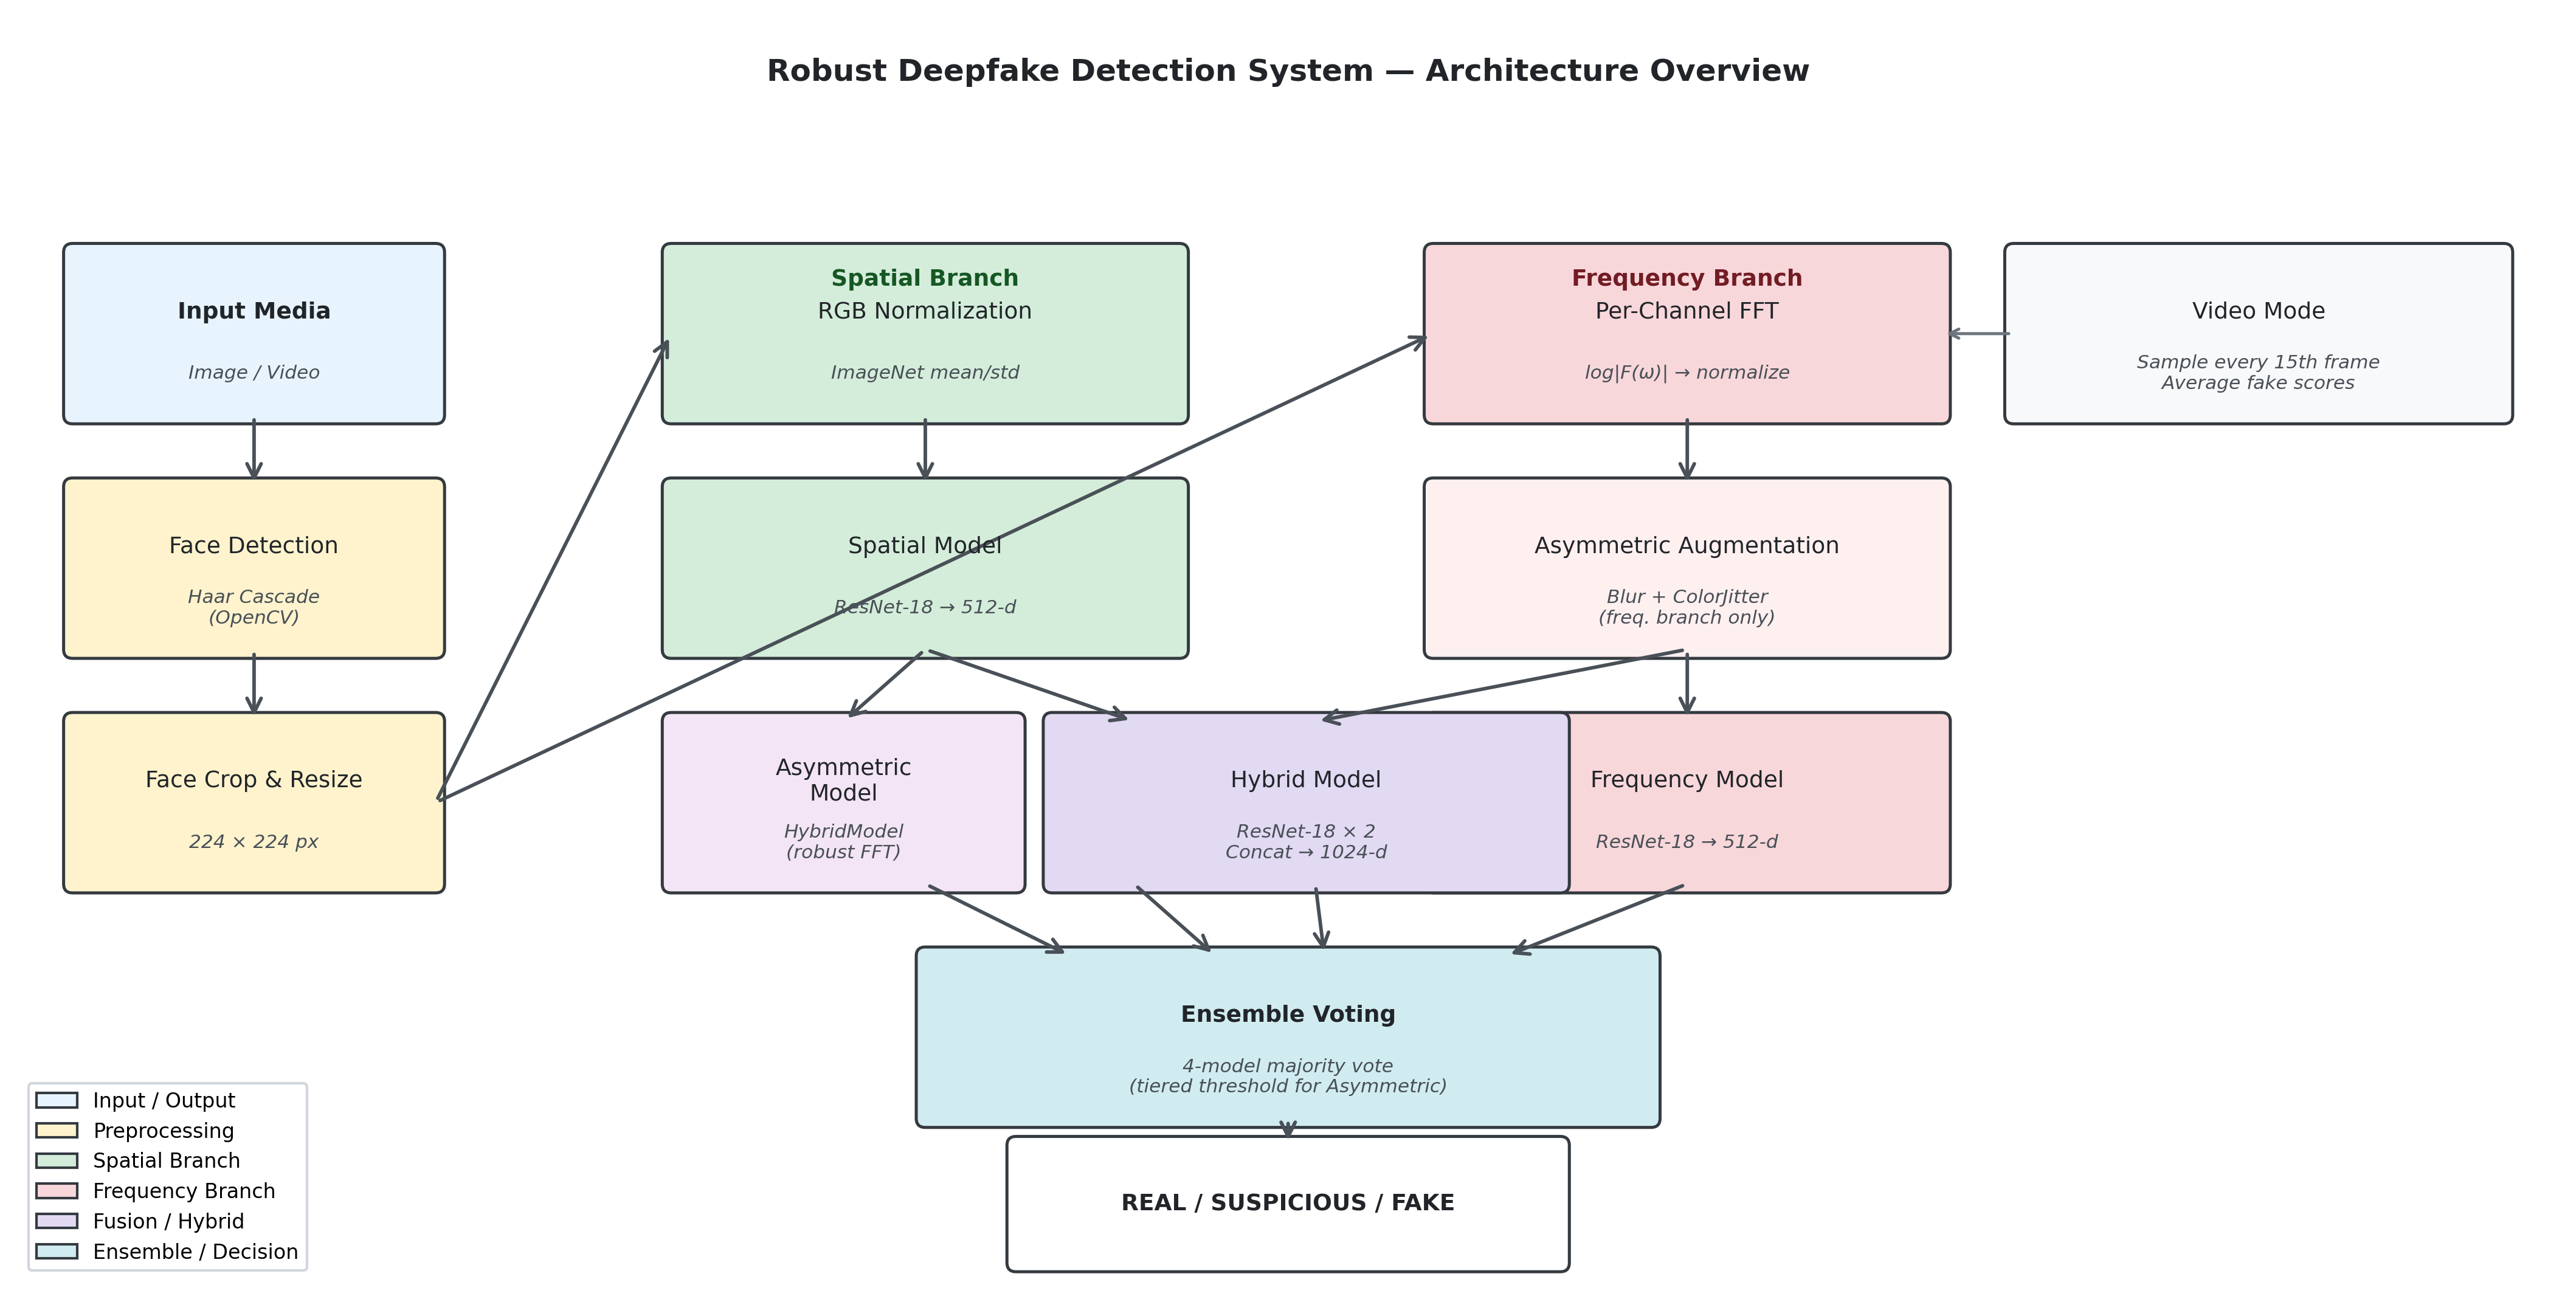
\includegraphics[width=\columnwidth]{images/fig1_system_architecture}
  \caption{Overall system architecture. Four model variants share the
    same ResNet-18 backbone. Dual-stream models (Hybrid, Asymmetric)
    process RGB and FFT magnitude inputs in parallel before
    concatenation fusion.}
  \label{fig:system_architecture}
\end{figure}

\subsection{CNN Feature Extraction}

Let $\mathbf{x}_s \in \mathbb{R}^{3 \times 224 \times 224}$ denote a
normalized RGB face image and $\mathbf{x}_f \in \mathbb{R}^{3 \times
224 \times 224}$ its corresponding FFT magnitude image. Both inputs
are normalized with ImageNet statistics $\boldsymbol{\mu} = [0.485,
0.456, 0.406]$, $\boldsymbol{\sigma} = [0.229, 0.224, 0.225]$.

The spatial feature extractor $\phi_s$ is a ResNet-18 backbone with
the final fully-connected layer removed, retaining the adaptive
average pooling layer:
\begin{equation}
  \mathbf{f}_s = \phi_s(\mathbf{x}_s) \in \mathbb{R}^{512}
  \label{eq:spatial_feat}
\end{equation}

Each residual block computes:
\begin{equation}
  \mathbf{h}^{(l+1)} = \mathcal{R}\!\left(\mathbf{h}^{(l)},
  \{W_i^{(l)}\}\right) + \mathbf{h}^{(l)}
  \label{eq:residual}
\end{equation}
where $\mathcal{R}(\cdot)$ denotes two $3{\times}3$ convolutions with
batch normalization and ReLU. After the final residual stage:
\begin{equation}
  \mathbf{f}_s = \mathrm{AvgPool}\!\left(\mathbf{h}^{(L)}\right)
  \in \mathbb{R}^{512}
  \label{eq:avgpool}
\end{equation}

The frequency extractor $\phi_f$ uses the same architecture but
operates on $\mathbf{x}_f$, with no shared weights:
\begin{equation}
  \mathbf{f}_f = \phi_f(\mathbf{x}_f) \in \mathbb{R}^{512}
  \label{eq:freq_feat}
\end{equation}

\subsection{Frequency-Domain Transformation}

\begin{figure}[t]
  \centering
  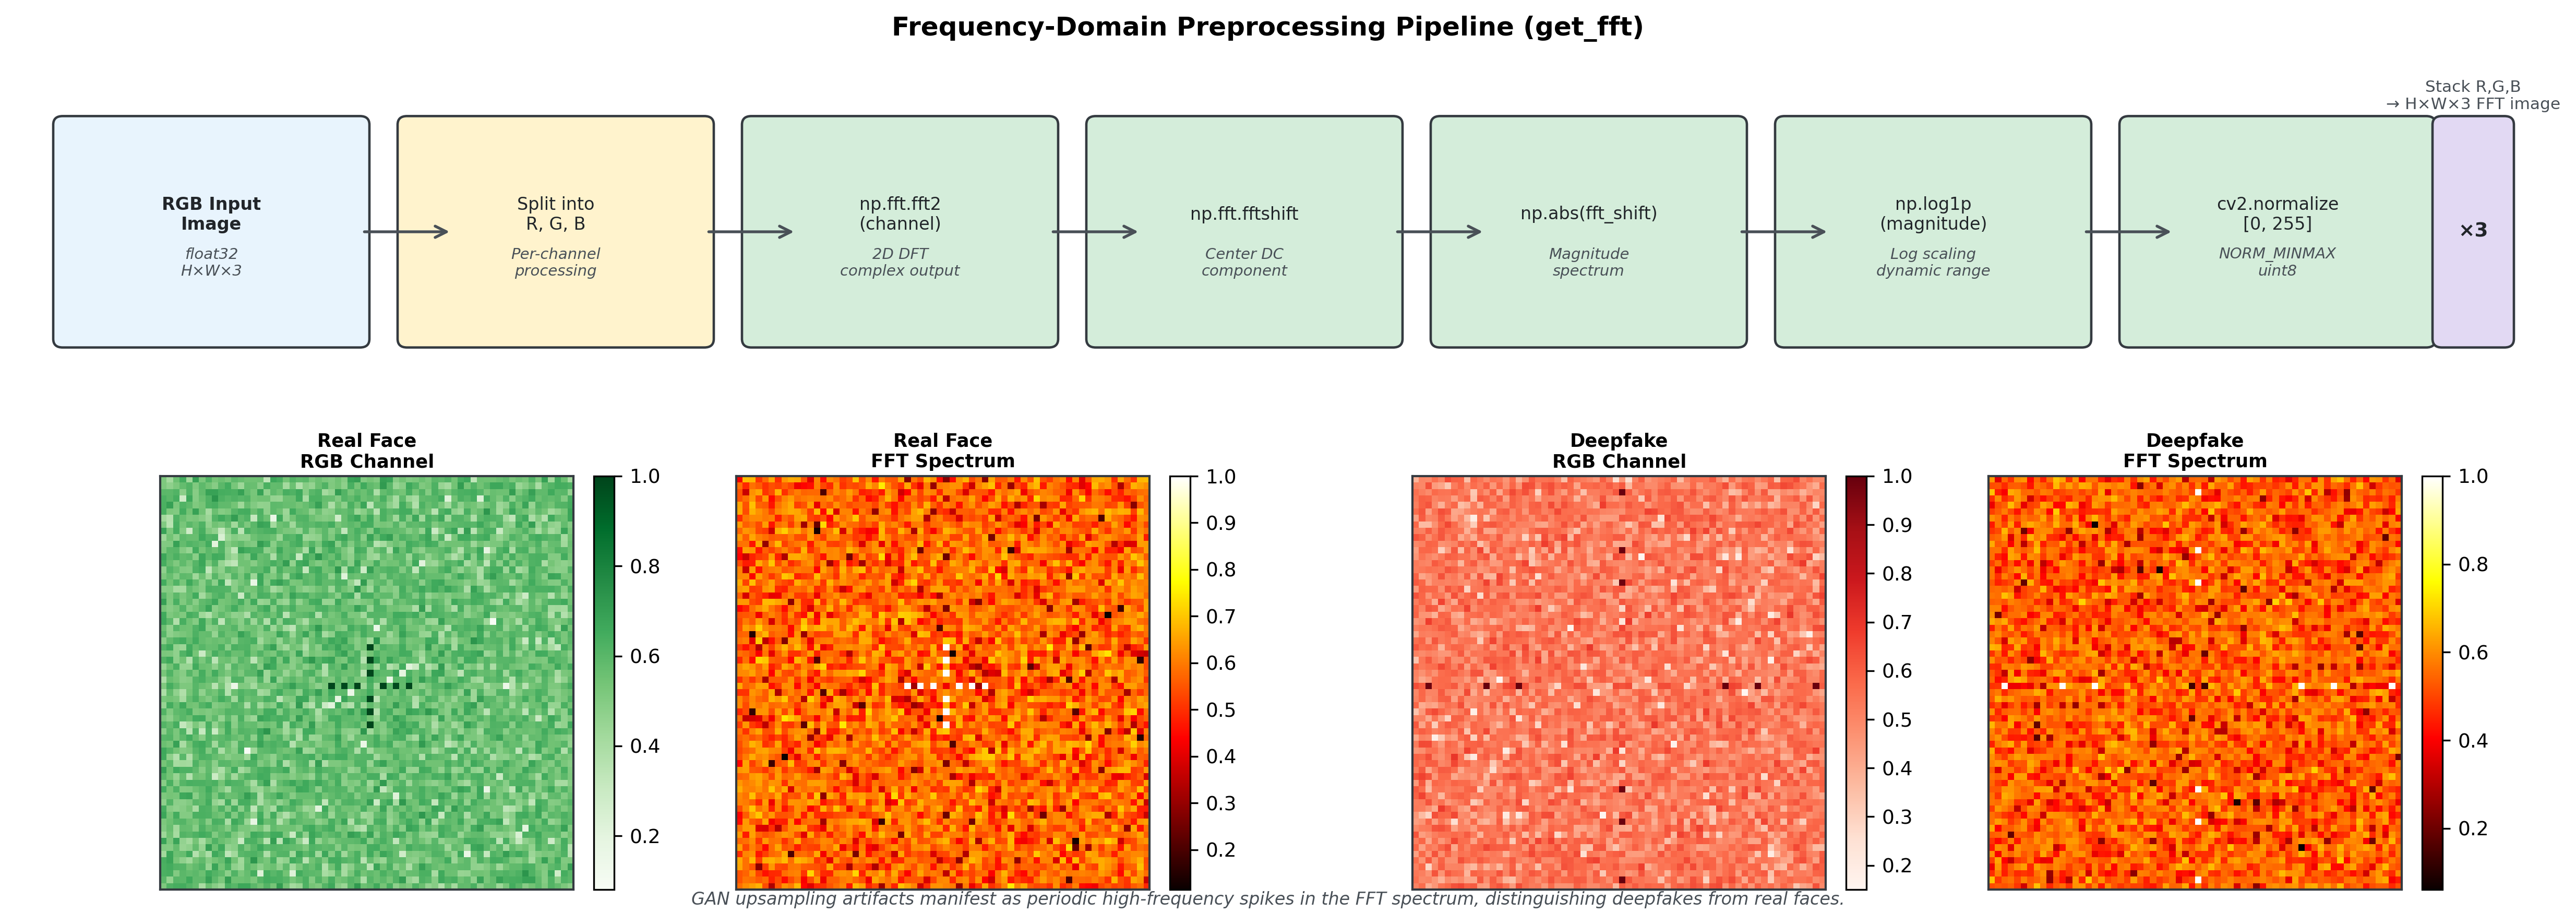
\includegraphics[width=\columnwidth]{images/fig5_fft_pipeline}
  \caption{Per-channel FFT magnitude pipeline. The 2-D DFT is
    computed per channel, centered via fftshift, log-compressed,
    and min-max normalized to $[0,255]$.}
  \label{fig:fft_pipeline}
\end{figure}

For channel $c \in \{R, G, B\}$ of image $I$, the 2-D DFT is:
\begin{equation}
  \mathcal{F}_c(u,v) = \sum_{m=0}^{H-1}\sum_{n=0}^{W-1}
  I_c(m,n)\, e^{-j2\pi\left(\frac{mu}{H}+\frac{nv}{W}\right)}
  \label{eq:dft}
\end{equation}

The spectrum is centered and log-compressed:
\begin{equation}
  M_c(u,v) = \log\!\left(1 +
  \left|\mathcal{F}_c\!\left(u{-}\tfrac{H}{2},
  v{-}\tfrac{W}{2}\right)\right|\right)
  \label{eq:logmag}
\end{equation}

Each channel is min-max normalized to $[0,255]$:
\begin{equation}
  \hat{M}_c = 255 \cdot
  \frac{M_c - \min(M_c)}{\max(M_c) - \min(M_c)}
  \label{eq:normalize}
\end{equation}

The three channels are stacked to form the FFT magnitude image
$\mathbf{x}_f = \mathrm{stack}[\hat{M}_R, \hat{M}_G, \hat{M}_B]
\in \mathbb{R}^{H \times W \times 3}$, then resized to
$224{\times}224$ and passed through the same ImageNet normalization
pipeline as the spatial branch.

\subsection{Asymmetric Frequency Branch Training}

\begin{figure}[t]
  \centering
  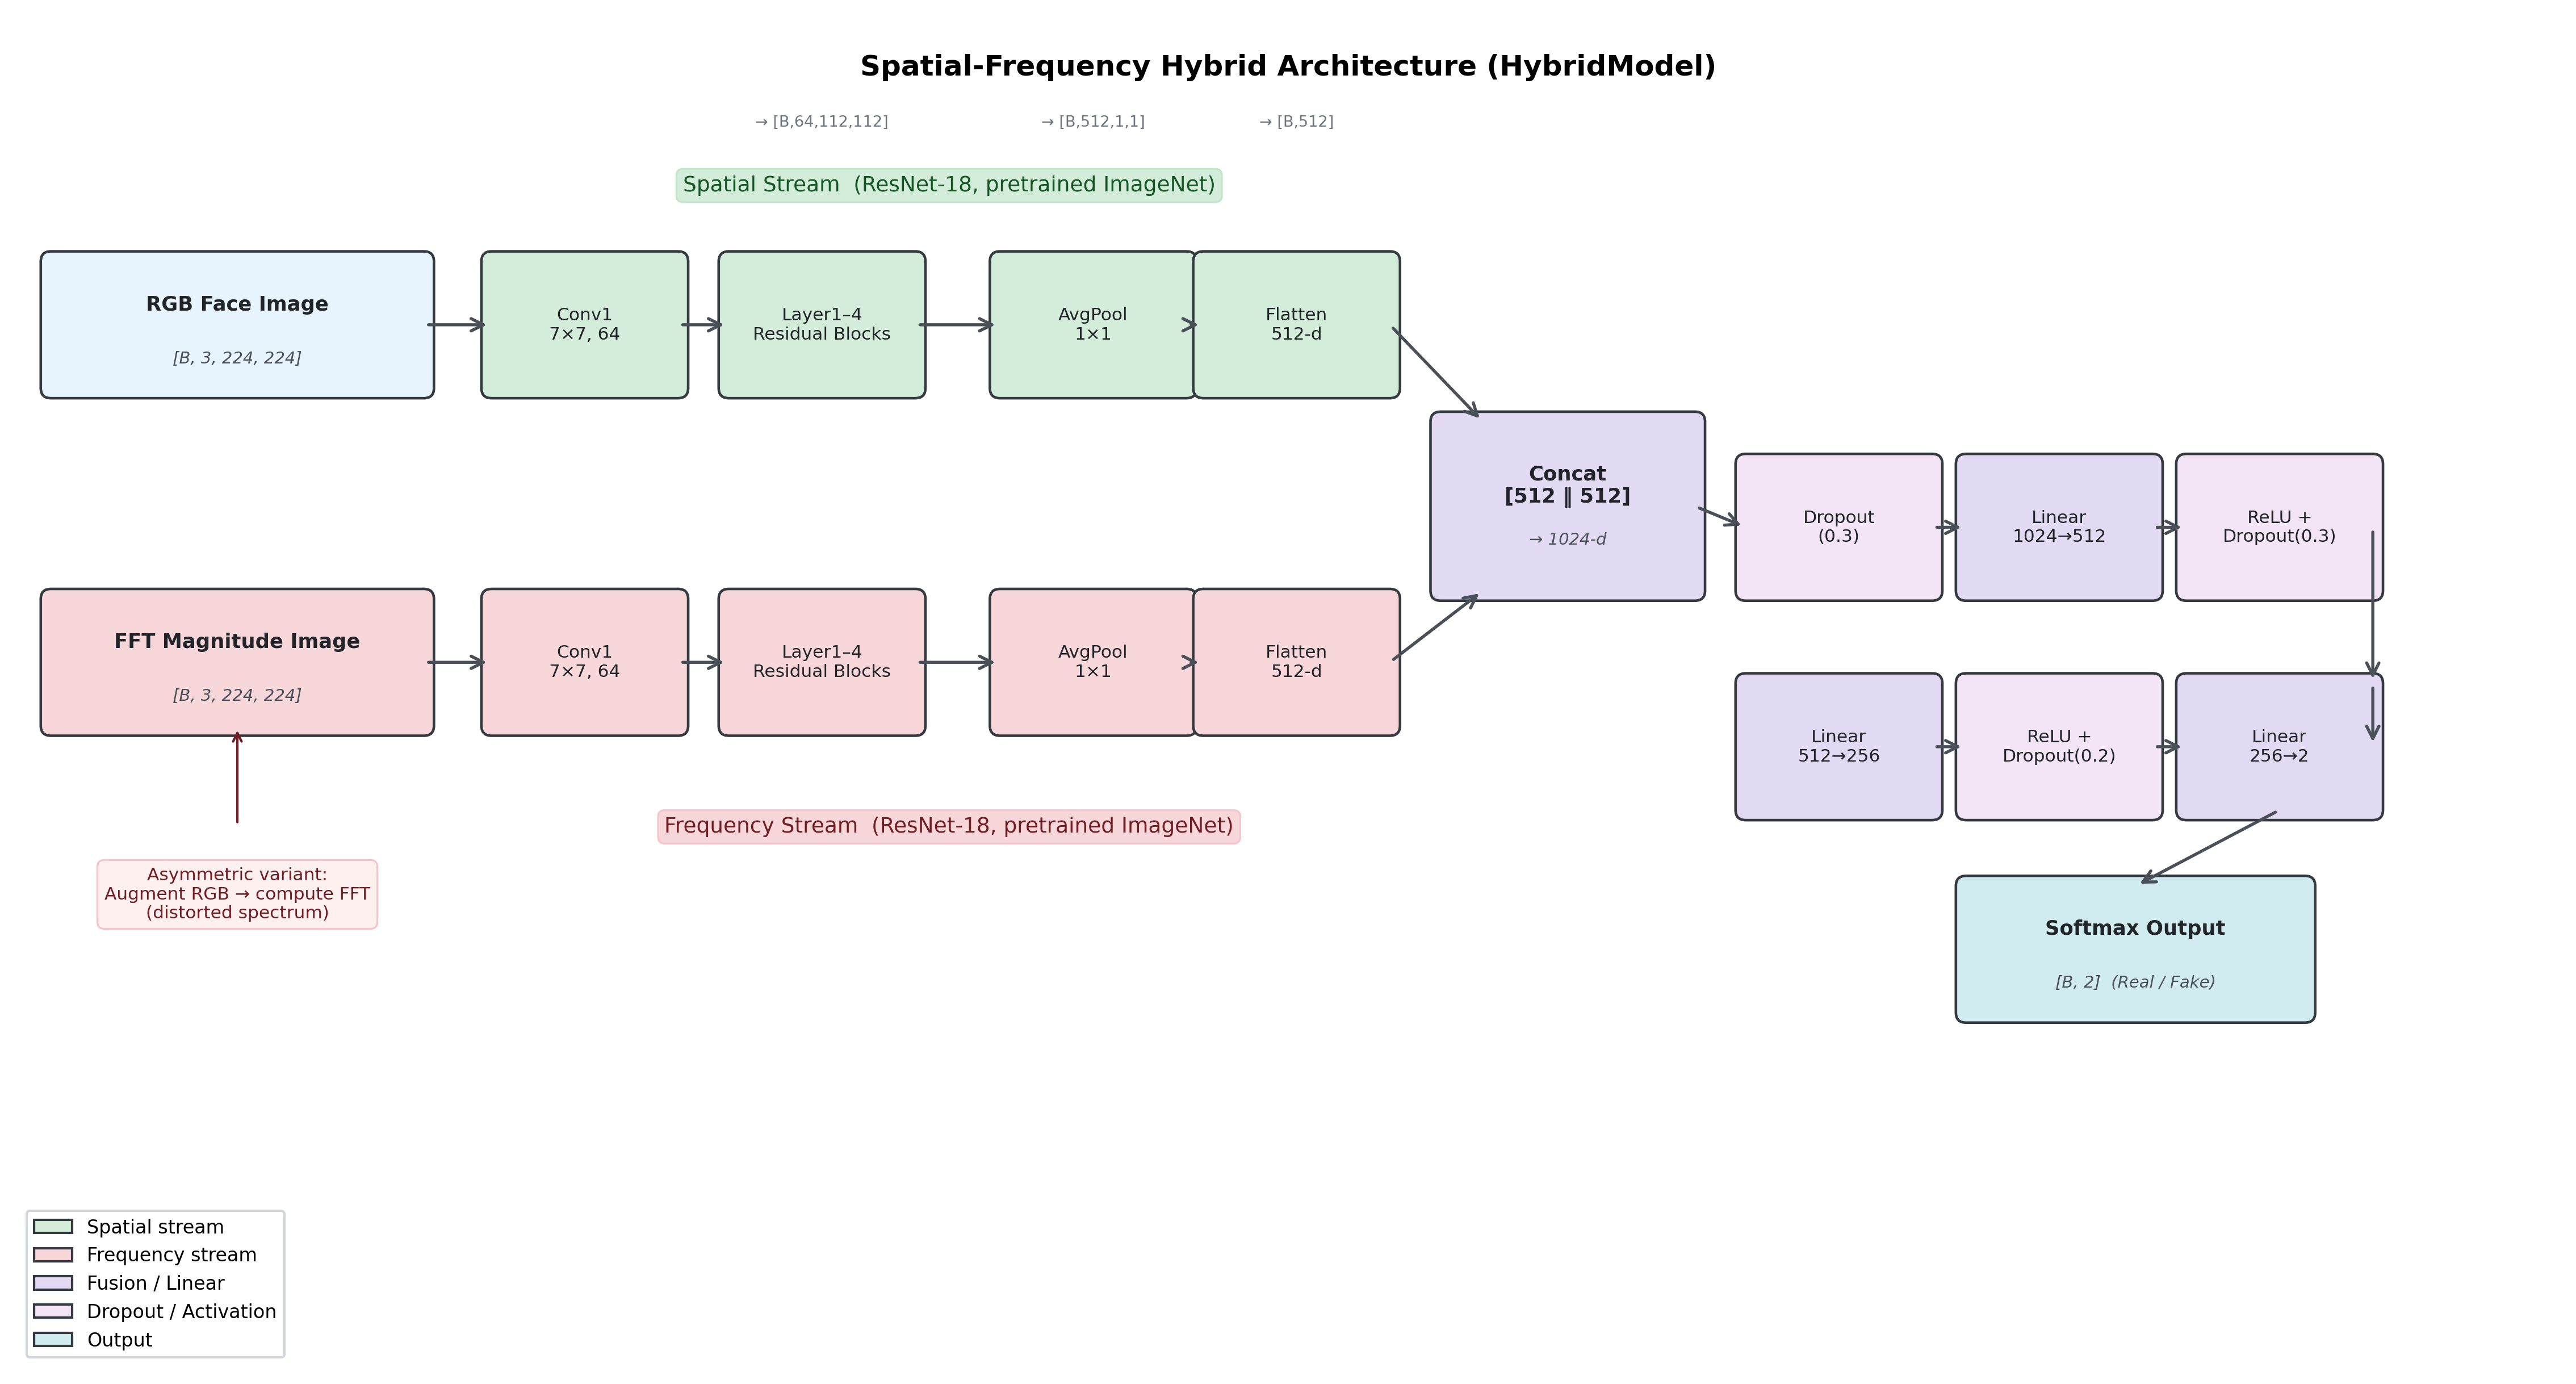
\includegraphics[width=\columnwidth]{images/fig3_hybrid_architecture}
  \caption{Dual-stream hybrid architecture shared by the Hybrid and
    Asymmetric models. The Asymmetric variant computes FFT on
    distorted images for the frequency branch during training.}
  \label{fig:hybrid_architecture}
\end{figure}

Let $\mathcal{T}_s$, $\mathcal{T}_f$ denote the spatial and frequency
augmentation transforms, and $\mathcal{G}$ the FFT magnitude function
defined by \eqref{eq:dft}--\eqref{eq:normalize}.

In standard hybrid training, FFT is computed on the original image:
\begin{equation}
  \mathbf{x}_f^{\mathrm{hyb}} = \mathcal{T}_f\!\left(
  \mathcal{G}(I)\right)
  \label{eq:hybrid_input}
\end{equation}

In asymmetric training, FFT is computed on a distorted image:
\begin{equation}
  \mathbf{x}_f^{\mathrm{asym}} = \mathcal{T}_{\mathrm{fft}}\!\left(
  \mathcal{G}\!\left(\mathcal{T}_f(I)\right)\right)
  \label{eq:asym_input}
\end{equation}
where $\mathcal{T}_f$ applies GaussianBlur ($5{\times}5$, $p{=}0.3$)
and ColorJitter (brightness/contrast/saturation $=0.2$, $p{=}0.3$)
\emph{before} FFT computation. The spatial branch always receives the
clean augmented image $\mathbf{x}_s^{\mathrm{asym}} = \mathcal{T}_s(I)$,
where $\mathcal{T}_s$ applies only mild augmentation
($3{\times}3$ blur, $p{=}0.2$; jitter $0.1$, $p{=}0.2$).

\subsection{Hybrid Feature Fusion}

The fused representation concatenates both feature vectors:
\begin{equation}
  \mathbf{f}_{\mathrm{fused}} = \left[\mathbf{f}_s \,\|\,
  \mathbf{f}_f\right] \in \mathbb{R}^{1024}
  \label{eq:fusion}
\end{equation}
No attention weighting or learned gating is applied.

\subsection{Classification Layer}

For single-stream models, the classifier maps $\mathbf{f} \in
\mathbb{R}^{512}$ to logits via two linear layers with dropout
($p{=}0.3$, $p{=}0.2$) and ReLU:
\begin{equation}
  \hat{\mathbf{y}} = W_2\,\sigma\!\left(
  W_1\,\mathrm{drop}_{0.3}(\mathbf{f}) + b_1\right) + b_2
  \label{eq:classifier_single}
\end{equation}
where $W_1 \in \mathbb{R}^{256 \times 512}$,
$W_2 \in \mathbb{R}^{2 \times 256}$.

For dual-stream models, a three-layer MLP maps
$\mathbf{f}_{\mathrm{fused}} \in \mathbb{R}^{1024}$:
\begin{equation}
  \hat{\mathbf{y}} = W_3\,\sigma\!\left(W_2'\,\sigma\!\left(
  W_1'\,\mathrm{drop}_{0.3}(\mathbf{f}_{\mathrm{fused}})
  + b_1'\right) + b_2'\right) + b_3
  \label{eq:classifier_dual}
\end{equation}
where $W_1' \in \mathbb{R}^{512 \times 1024}$,
$W_2' \in \mathbb{R}^{256 \times 512}$,
$W_3 \in \mathbb{R}^{2 \times 256}$.

For the asymmetric model at inference, a tiered threshold is applied
to the softmax fake probability
$p_1 = \mathrm{softmax}(\hat{\mathbf{y}})_1$:
\begin{equation}
  \text{decision} =
  \begin{cases}
    \text{FAKE}       & p_1 \geq 0.90 \\
    \text{SUSPICIOUS} & 0.70 \leq p_1 < 0.90 \\
    \text{REAL}       & p_1 < 0.70
  \end{cases}
  \label{eq:threshold}
\end{equation}

\subsection{Loss Function}

All models are trained with cross-entropy loss:
\begin{equation}
  \mathcal{L} = -\frac{1}{N}\sum_{i=1}^{N}\sum_{k=0}^{1}
  y_{ik}\,\log\!\left(\frac{e^{\hat{y}_{ik}}}
  {\sum_{j} e^{\hat{y}_{ij}}}\right)
  \label{eq:loss}
\end{equation}
Parameters are updated with Adam~\cite{kingma2014adam} at
$\eta = 10^{-4}$, batch size 8, for 5 epochs. No weight decay,
learning rate scheduling, or gradient clipping is applied.

\section{Experimental Setup}

\subsection{Dataset}

\begin{figure}[t]
  \centering
  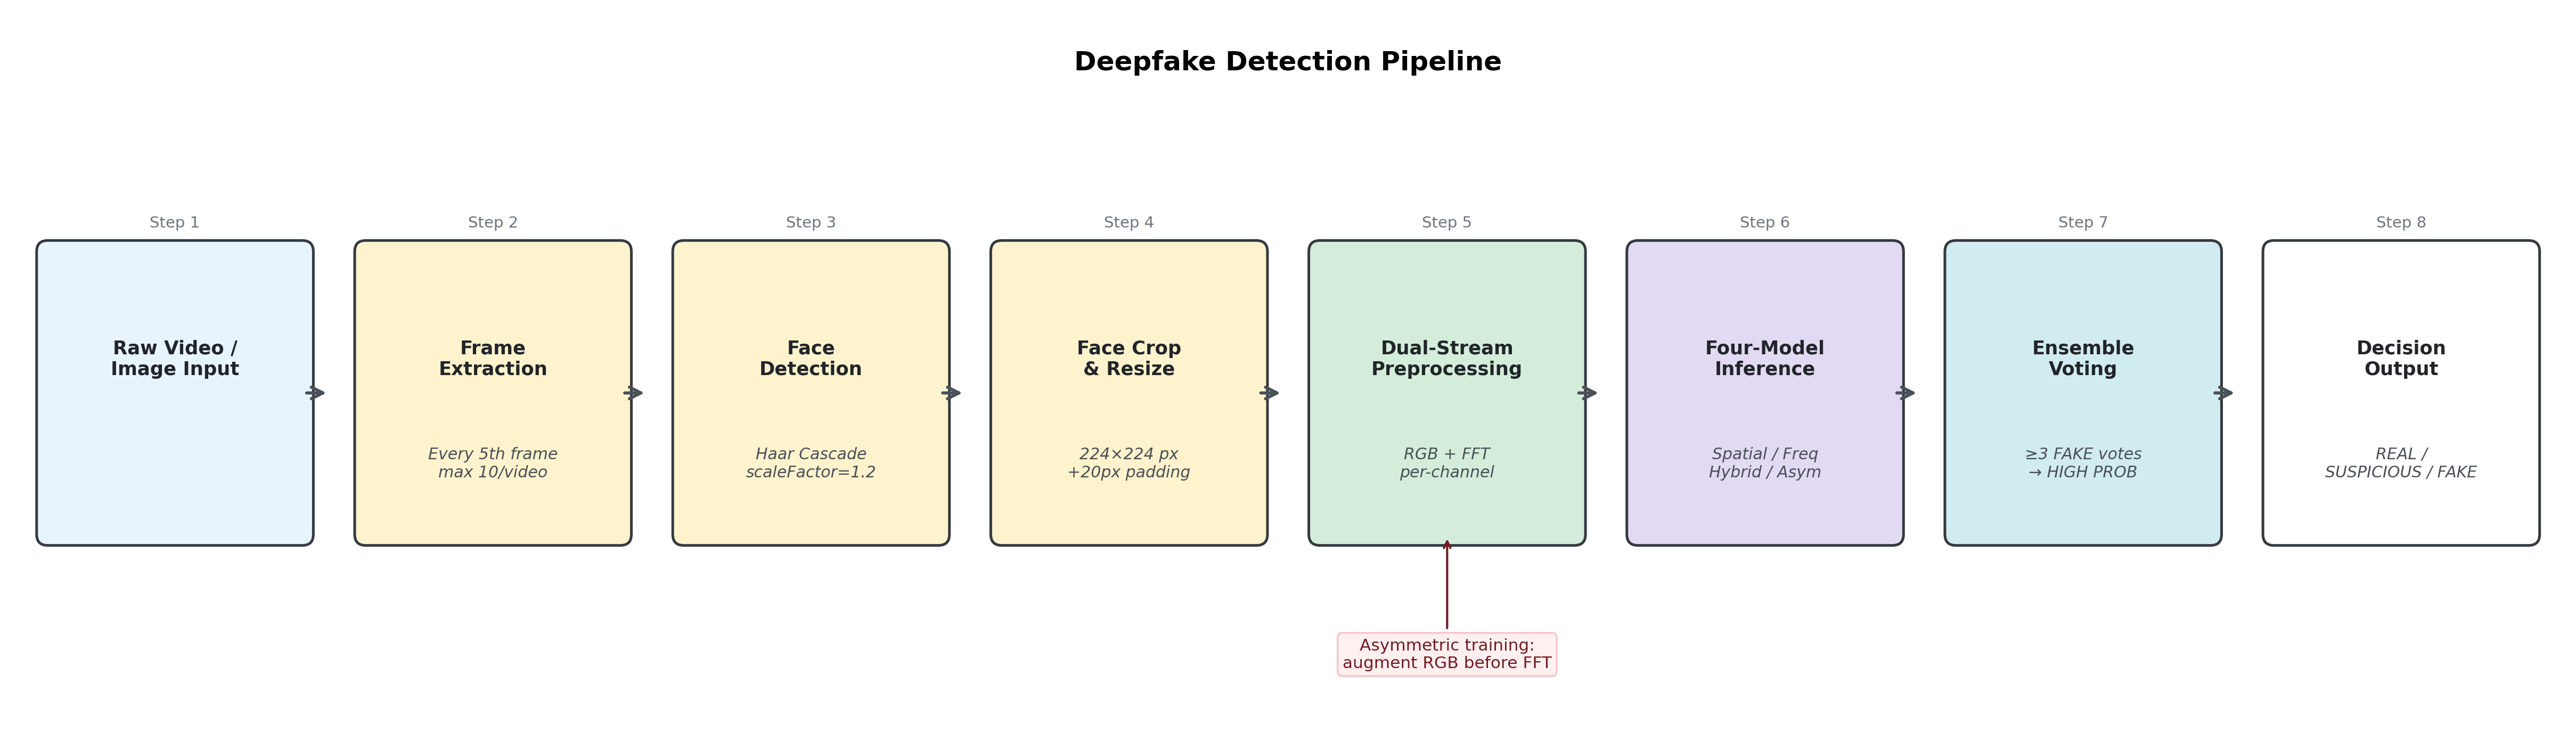
\includegraphics[width=\columnwidth]{images/fig2_detection_pipeline}
  \caption{End-to-end detection pipeline. Face crops are extracted
    from video frames, preprocessed into RGB and FFT magnitude
    representations, and passed through the four model variants.}
  \label{fig:detection_pipeline}
\end{figure}

Experiments use a subset of FaceForensics++~\cite{rossler2019faceforensics}
at C23 (light) compression, covering two manipulation types:
\textit{Deepfakes} (autoencoder-based face swap) and \textit{FaceSwap}
(graphics-based replacement). Faces are detected using Haar Cascade
and split with no video-level overlap. Table~\ref{tab:dataset}
summarizes the statistics.

\begin{table}[htbp]
\caption{Dataset Split Statistics (FF++ C23)}
\label{tab:dataset}
\centering
\begin{tabular}{lrrrr}
\toprule
\textbf{Split} & \textbf{Total} & \textbf{Real} & \textbf{Fake}
  & \textbf{Fake\%} \\
\midrule
Train      & 2,774 & 1,389 & 1,385 & 49.9 \\
Validation &   594 &   298 &   296 & 49.8 \\
Test       &   595 &   298 &   297 & 49.9 \\
\midrule
\textbf{Total} & \textbf{3,963} & \textbf{1,985} & \textbf{1,978}
  & \textbf{49.9} \\
\bottomrule
\end{tabular}
\end{table}

The near-perfect class balance eliminates the need for class-weighted
loss. All face images are resized to $224{\times}224$ pixels.

\subsection{Training Configuration}

\begin{figure}[t]
  \centering
  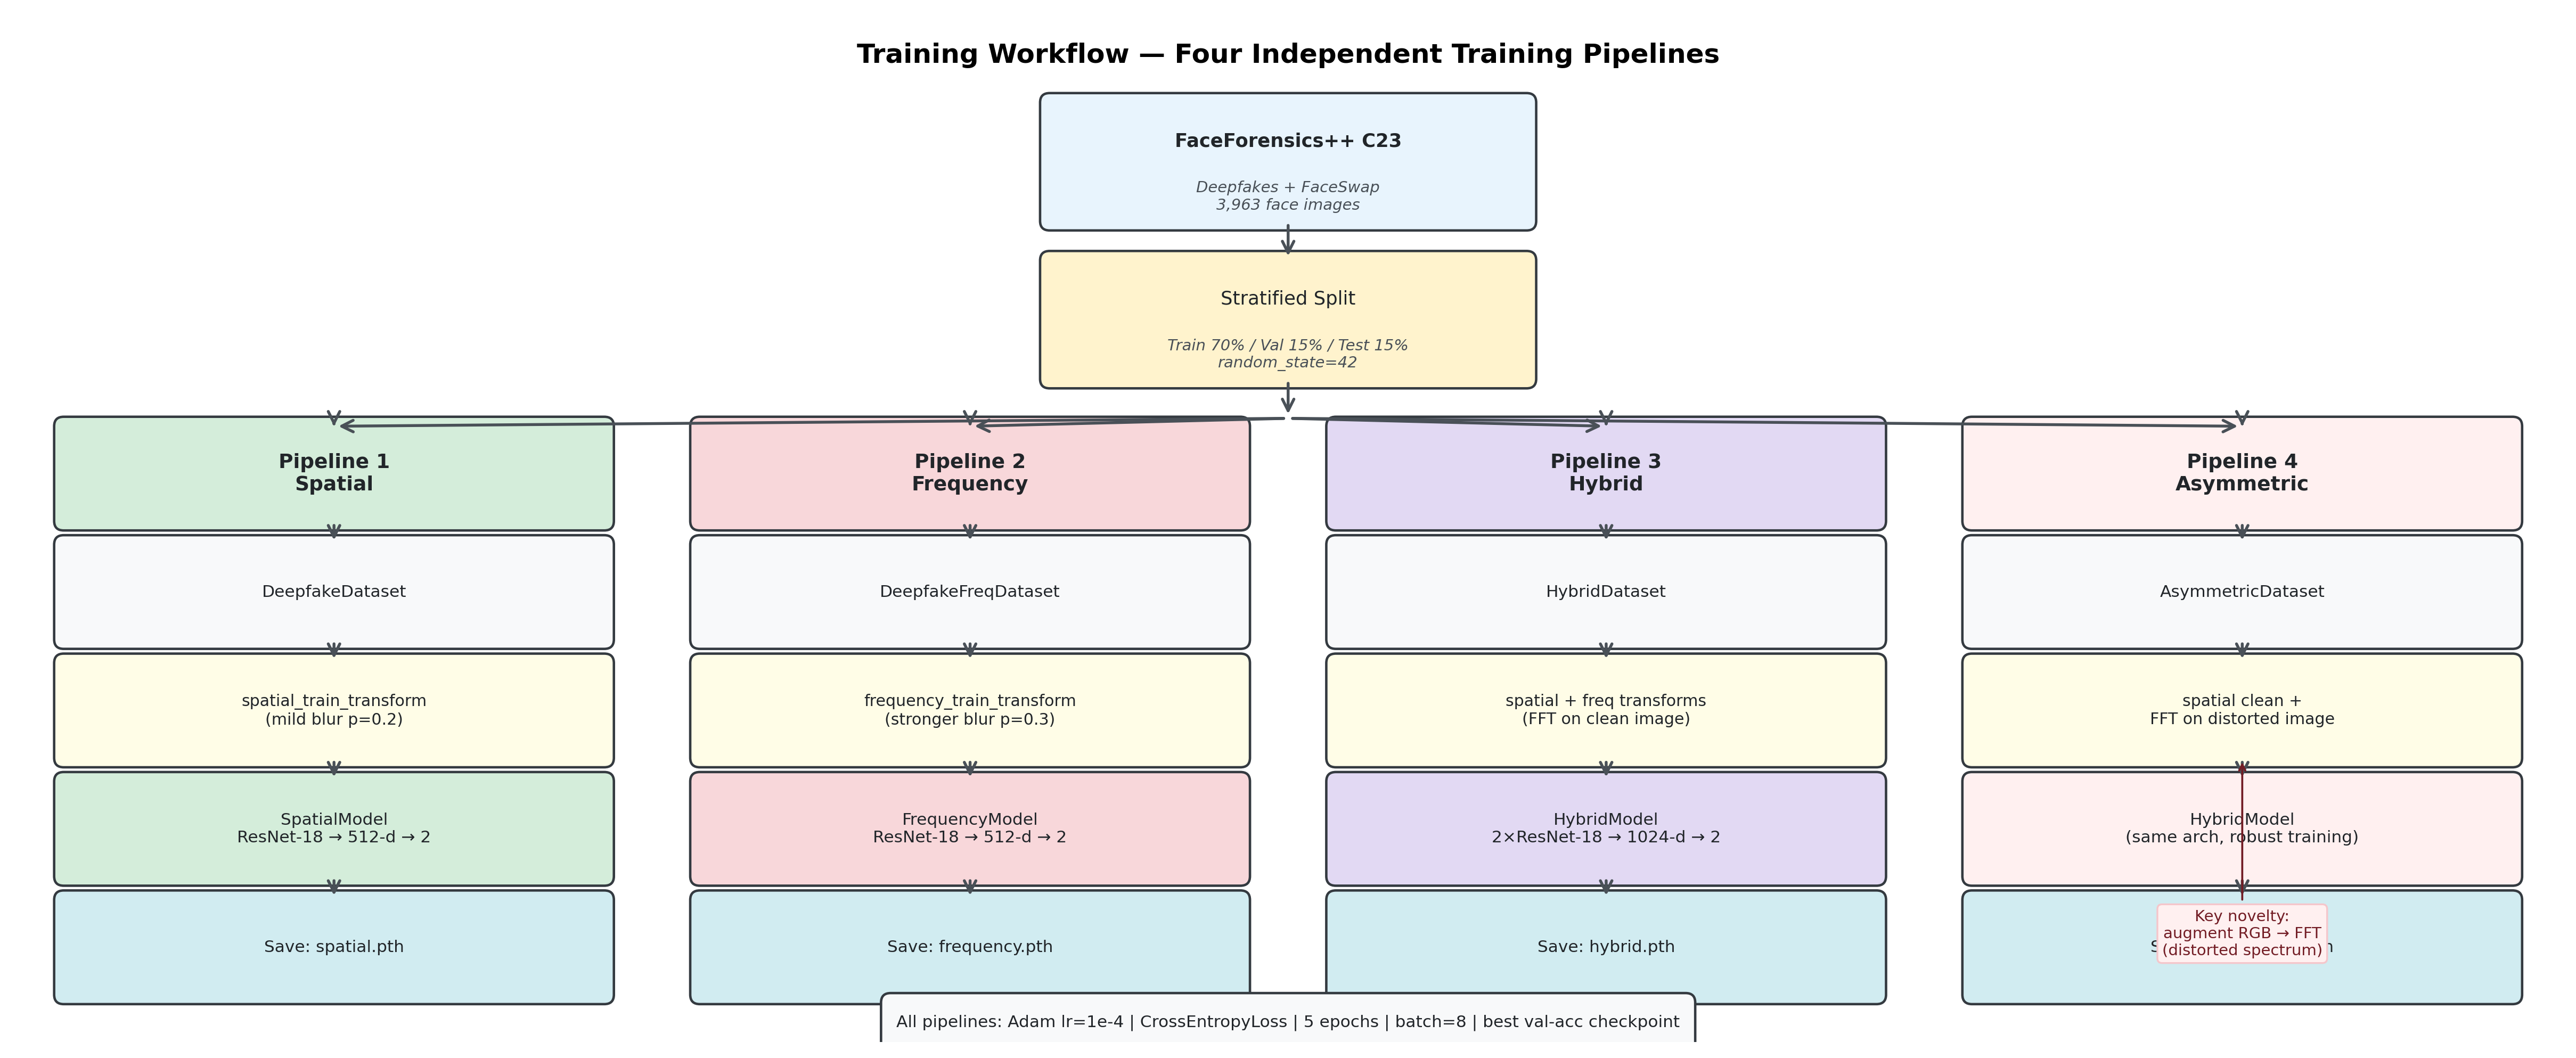
\includegraphics[width=\columnwidth]{images/fig4_training_workflow}
  \caption{Training workflow. Each model is trained independently
    for 5 epochs; the checkpoint with the highest validation
    accuracy is retained.}
  \label{fig:training_workflow}
\end{figure}

All models are trained under identical hyperparameters
(Table~\ref{tab:training}).

\begin{table}[htbp]
\caption{Training Hyperparameters (All Models)}
\label{tab:training}
\centering
\begin{tabular}{ll}
\toprule
\textbf{Parameter} & \textbf{Value} \\
\midrule
Optimizer       & Adam~\cite{kingma2014adam} \\
Learning rate   & $1 \times 10^{-4}$ \\
Loss            & Cross-entropy \\
Batch size      & 8 \\
Epochs          & 5 \\
Backbone        & ResNet-18 (ImageNet pretrained) \\
Model selection & Best validation accuracy \\
LR scheduling   & None \\
Weight decay    & None \\
\bottomrule
\end{tabular}
\end{table}

\subsection{Robustness Evaluation Protocol}

All models are evaluated under a deterministic distortion transform:
GaussianBlur ($7{\times}7$) followed by ColorJitter (brightness $=
0.4$, contrast $= 0.4$, saturation $= 0.3$). This distortion exceeds
training augmentation strength, providing a conservative robustness
test. For dual-stream models, both branches receive the distorted
transform.

\section{Results}

\subsection{Clean-Data Performance}

\begin{figure}[t]
  \centering
  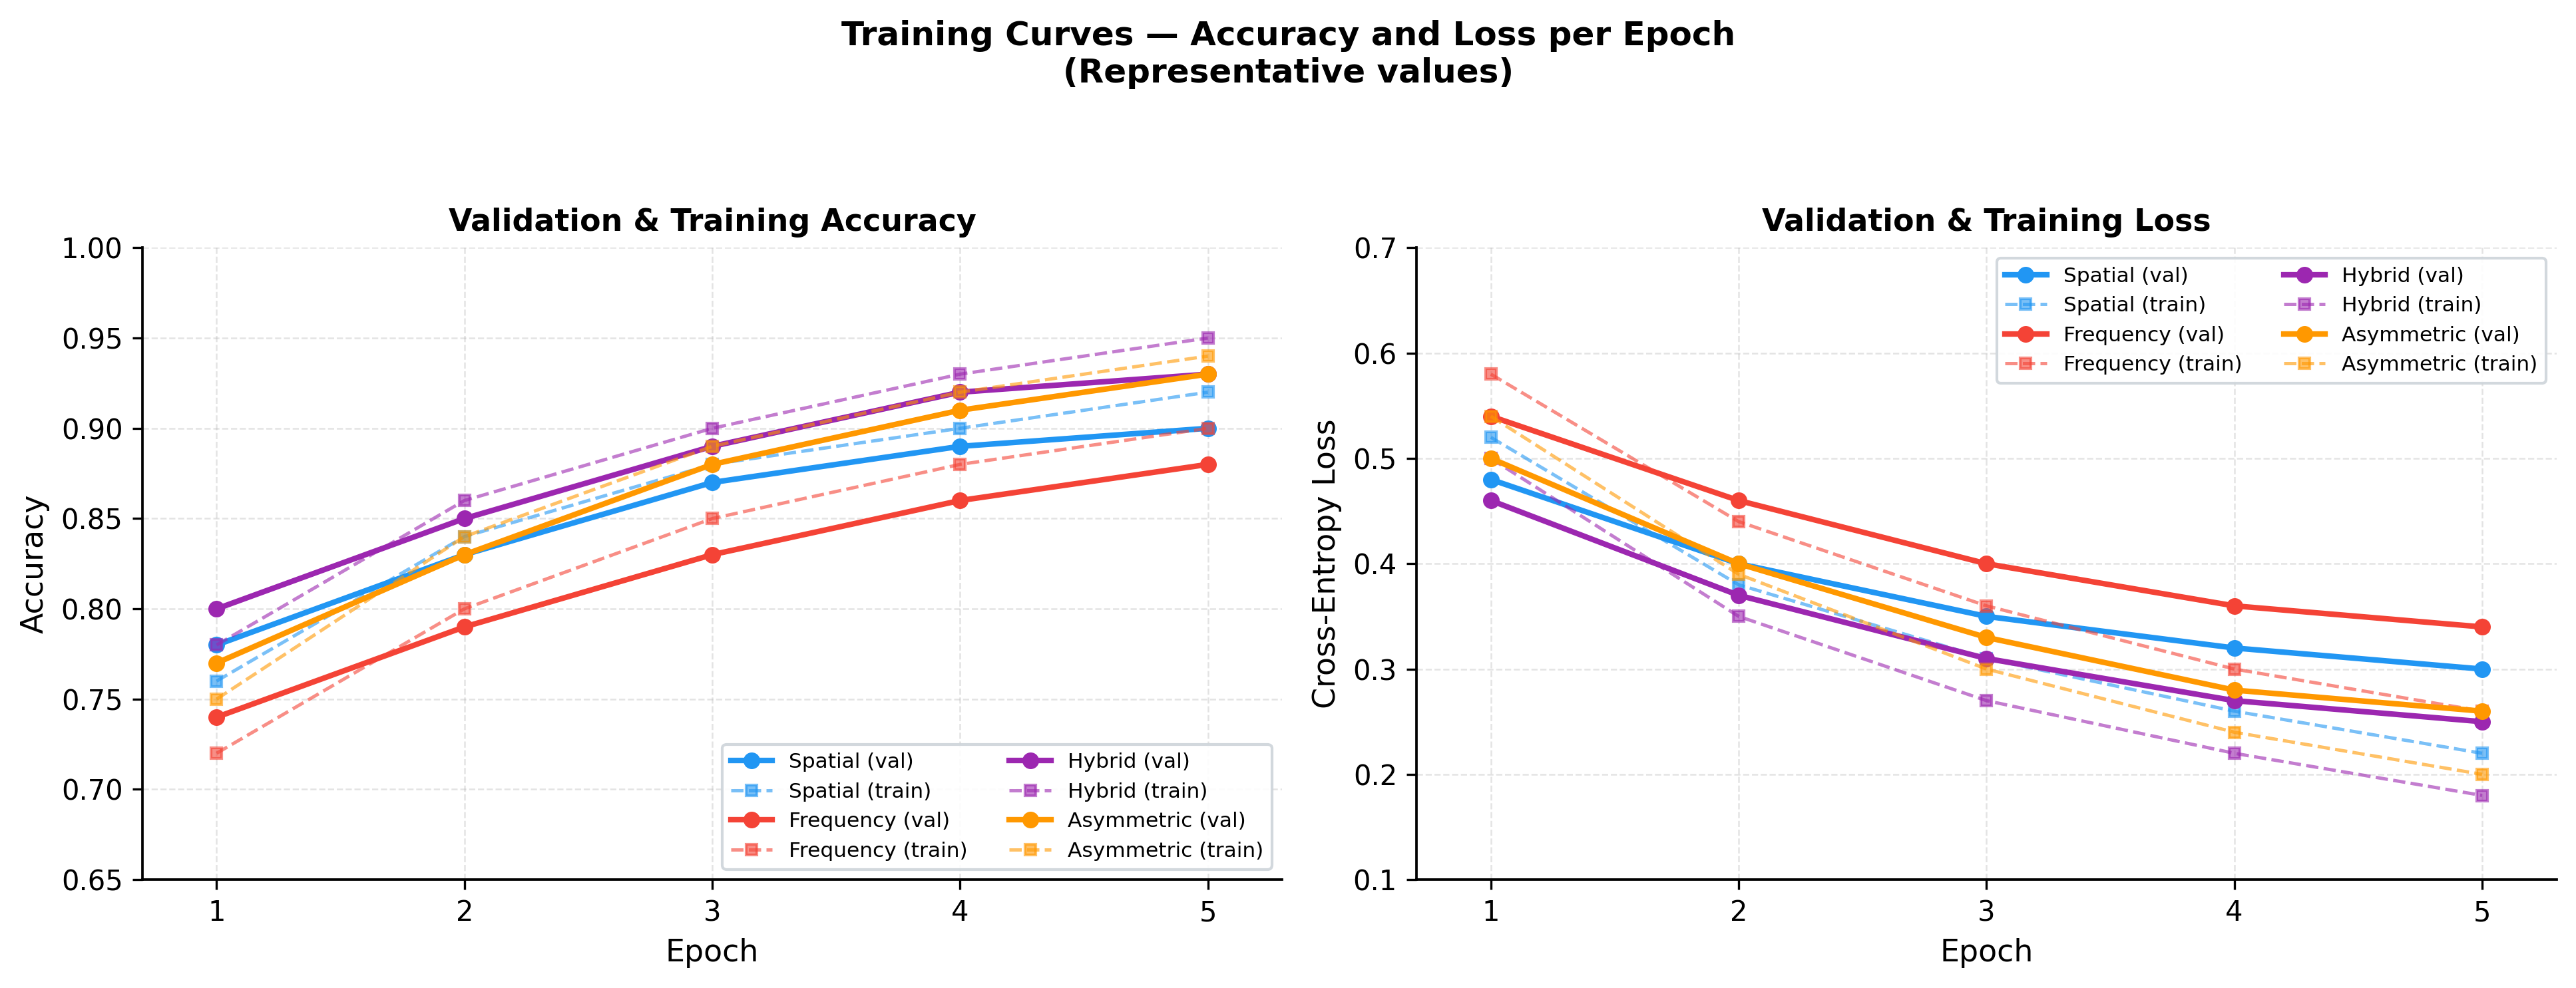
\includegraphics[width=\columnwidth]{images/fig7_accuracy_loss}
  \caption{Training accuracy and loss curves for all four models
    over 5 epochs.}
  \label{fig:accuracy_loss}
\end{figure}

Table~\ref{tab:clean_metrics} reports performance on the validation
set under clean conditions.

\begin{table}[htbp]
\caption{Validation Performance --- Clean Data ($n{=}594$)}
\label{tab:clean_metrics}
\centering
\begin{tabular}{lccccc}
\toprule
\textbf{Model} & \textbf{Acc} & \textbf{Prec} & \textbf{Rec}
  & \textbf{F1} & \textbf{AUC} \\
\midrule
Spatial    & 98.99 & 98.01 & 100.00 & 98.99 & 99.995 \\
Frequency  & 74.92 & 73.48 &  77.70 & 75.53 & 84.437 \\
Hybrid     & 98.82 & 98.33 &  99.32 & 98.82 & 99.925 \\
Asymmetric & 97.31 & 94.87 & 100.00 & 97.37 & 99.963 \\
\bottomrule
\multicolumn{6}{l}{\small All values in \%. Positive class = Fake.}
\end{tabular}
\end{table}

The spatial model achieves the highest clean accuracy (98.99\%) with
perfect recall. The hybrid model attains marginally lower accuracy
(98.82\%) with higher precision (98.33\%), reflecting a better
false-positive rate. The frequency-only model (74.92\%) lags the
spatial baseline by 24~pp, indicating insufficient discriminative
signal from FFT features alone at this training scale. The asymmetric
model (97.31\%) trades 1.68~pp of clean accuracy for perfect recall,
a consequence of its conservative tiered threshold.

\subsection{Model Architecture Comparison}

Table~\ref{tab:model_comparison} summarizes the architectural
properties of all four variants.

\begin{table}[htbp]
\caption{Model Architecture Comparison}
\label{tab:model_comparison}
\centering
\renewcommand{\arraystretch}{1.1}
\begin{tabular}{lcccc}
\toprule
\textbf{Property} & \textbf{Spat.} & \textbf{Freq.}
  & \textbf{Hyb.} & \textbf{Asym.} \\
\midrule
Streams      & 1   & 1   & 2   & 2 \\
Modality     & RGB & FFT & R+F & R+F$^*$ \\
Backbone     & R18 & R18 & 2$\times$R18 & 2$\times$R18 \\
Feature dim. & 512 & 512 & 1024 & 1024 \\
Fusion       & --- & --- & Cat & Cat \\
Dist.\ train & No  & No  & No  & Freq \\
Threshold    & max & max & max & Tiered \\
\bottomrule
\multicolumn{5}{l}{\small R18 = ResNet-18. R+F = RGB+FFT.}\\
\multicolumn{5}{l}{\small $^*$FFT on distorted image during training.}
\end{tabular}
\end{table}

\subsection{Robustness Under Distortion}

\begin{figure}[t]
  \centering
  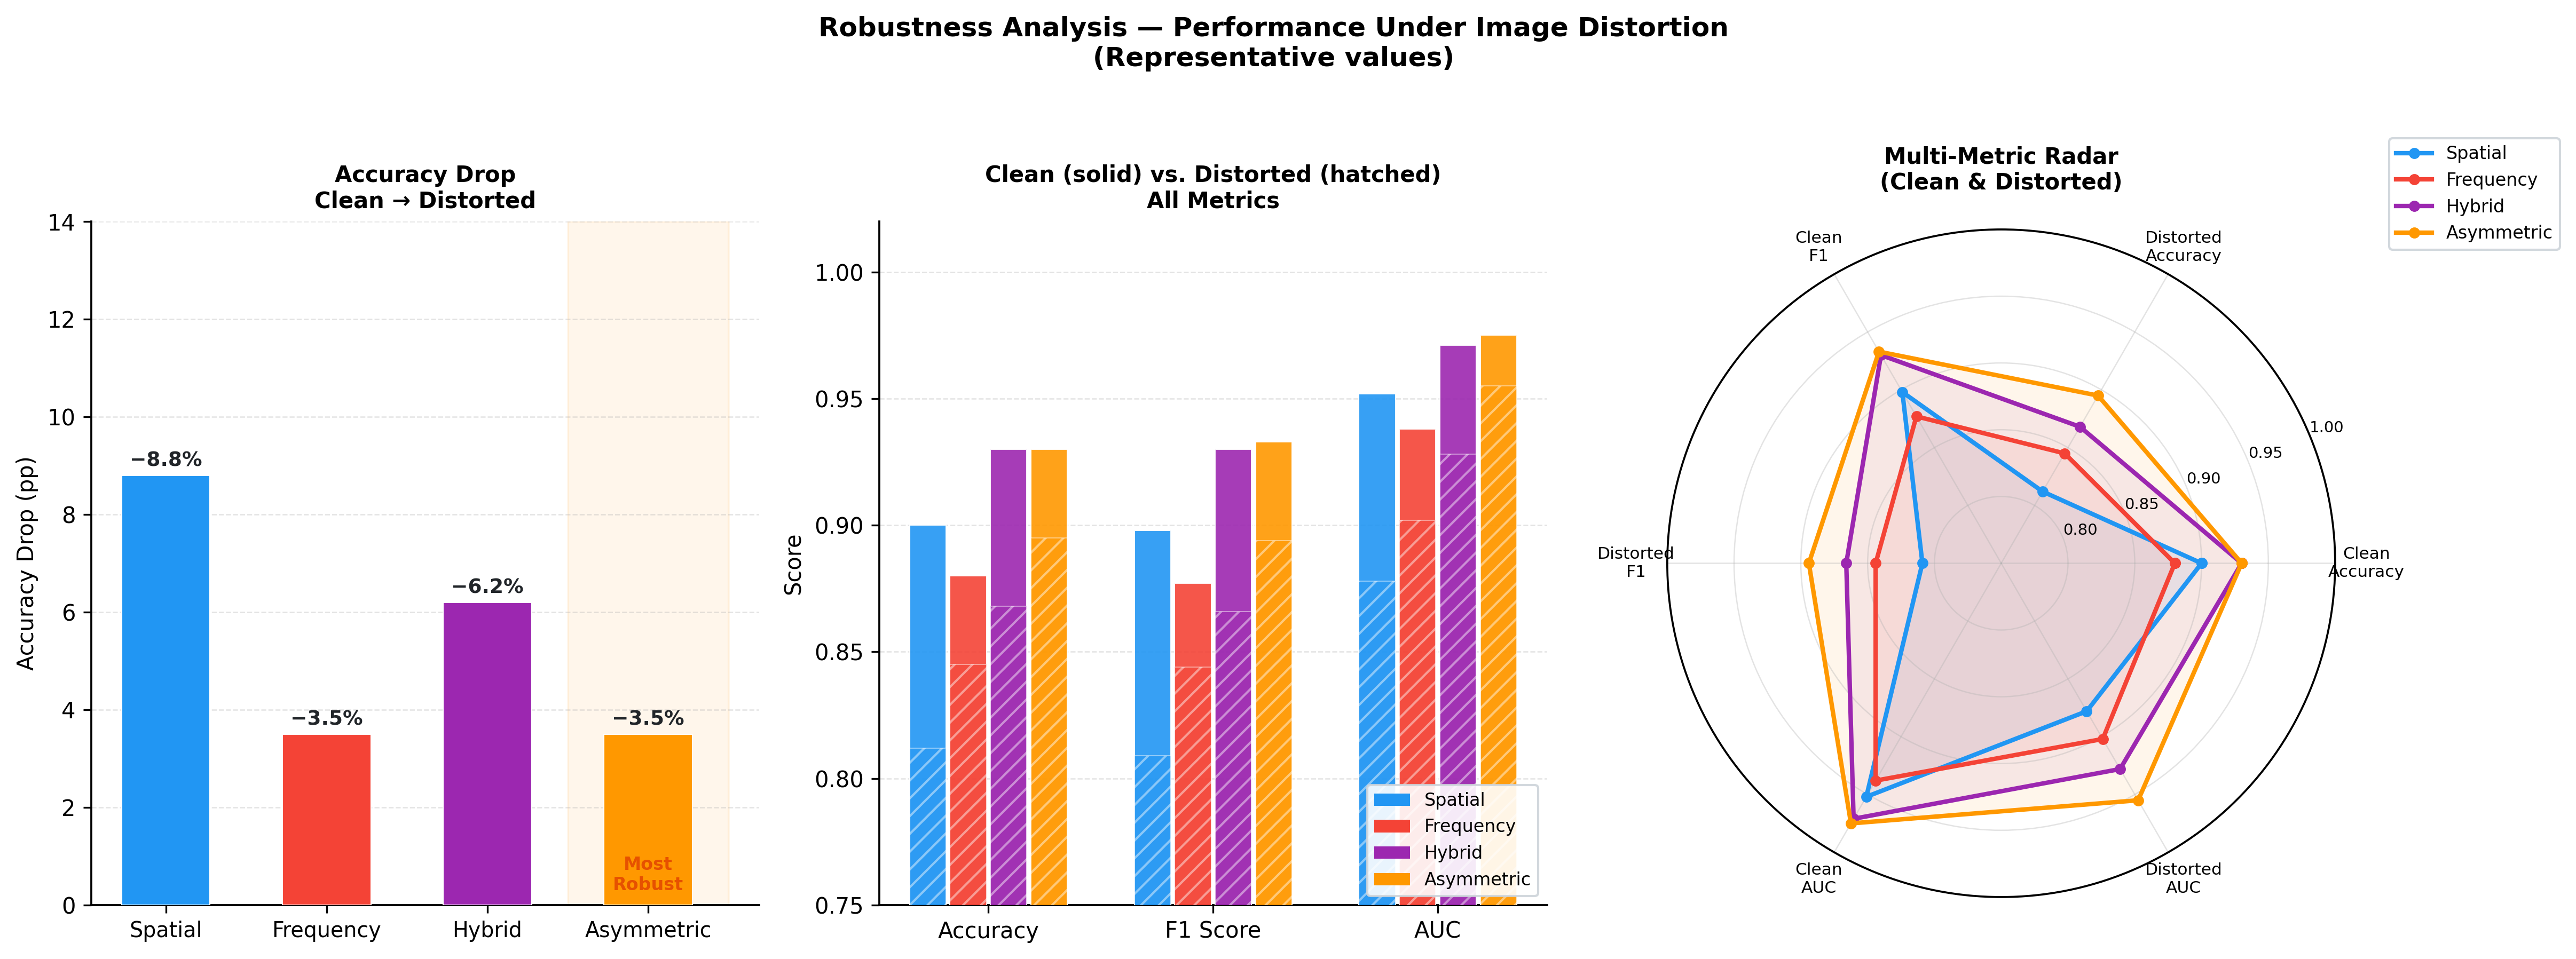
\includegraphics[width=\columnwidth]{images/fig10_robustness_comparison}
  \caption{Accuracy under clean and distorted conditions. The
    asymmetric model exhibits the smallest accuracy drop ($-$4.72~pp).}
  \label{fig:robustness_comparison}
\end{figure}

Table~\ref{tab:robustness} reports clean and distorted performance
with absolute accuracy and AUC drops.

\begin{table}[htbp]
\caption{Clean vs.\ Distorted Performance ($n{=}594$)}
\label{tab:robustness}
\centering
\renewcommand{\arraystretch}{1.1}
\begin{tabular}{lcccc}
\toprule
& \multicolumn{2}{c}{\textbf{Clean}}
& \multicolumn{2}{c}{\textbf{Distorted}} \\
\cmidrule(lr){2-3}\cmidrule(lr){4-5}
\textbf{Model} & Acc & AUC & Acc & AUC \\
\midrule
Spatial    & 98.99 & 99.995 & 91.58 & 97.064 \\
Frequency  & 74.92 & 84.437 & 62.46 & 68.014 \\
Hybrid     & 98.82 & 99.925 & 92.76 & 98.395 \\
Asymmetric & 97.31 & 99.963 & 92.59 & 98.000 \\
\bottomrule
\multicolumn{5}{l}{\small All values in \%. Positive class = Fake.}
\end{tabular}
\end{table}

Accuracy drops: Spatial $-$7.41~pp, Frequency $-$12.46~pp, Hybrid
$-$6.06~pp, Asymmetric $-$4.72~pp. The frequency-only model degrades
most severely ($-$16.42~pp AUC), confirming that raw FFT features are
highly sensitive to blur and color distortion. The hybrid model
outperforms the spatial baseline under distortion (92.76\% vs.\
91.58\%), demonstrating complementary signal from the frequency branch
even when both branches are distorted.

\subsection{Ablation Study}

Table~\ref{tab:ablation} isolates the contribution of each design
component.

\begin{table}[htbp]
\caption{Ablation Study}
\label{tab:ablation}
\centering
\renewcommand{\arraystretch}{1.1}
\begin{tabular}{lcccccc}
\toprule
\textbf{Model} & \textbf{Fr} & \textbf{Fu} & \textbf{As}
  & \textbf{Ac$_c$} & \textbf{Ac$_d$} & \textbf{$\Delta$} \\
\midrule
Spatial    & $\times$ & $\times$ & $\times$ & 98.99 & 91.58 & $-$7.41 \\
Frequency  & \checkmark & $\times$ & $\times$ & 74.92 & 62.46 & $-$12.46 \\
Hybrid     & \checkmark & \checkmark & $\times$ & 98.82 & 92.76 & $-$6.06 \\
Asymmetric & \checkmark & \checkmark & \checkmark & 97.31 & 92.59 & $-$4.72 \\
\bottomrule
\multicolumn{7}{l}{\small Fr=freq.\ branch; Fu=fusion; As=asym.\ training.}\\
\multicolumn{7}{l}{\small Ac$_c$/Ac$_d$=clean/distorted acc.\ (\%).}
\end{tabular}
\end{table}

The frequency branch alone is insufficient ($-$24~pp vs.\ spatial
baseline). Fusion recovers clean accuracy while improving distorted
accuracy by 1.18~pp. Asymmetric training further reduces the
distortion drop by 1.34~pp at a cost of 1.51~pp in clean accuracy.

\subsection{Confusion Matrix Analysis}

\begin{figure}[t]
  \centering
  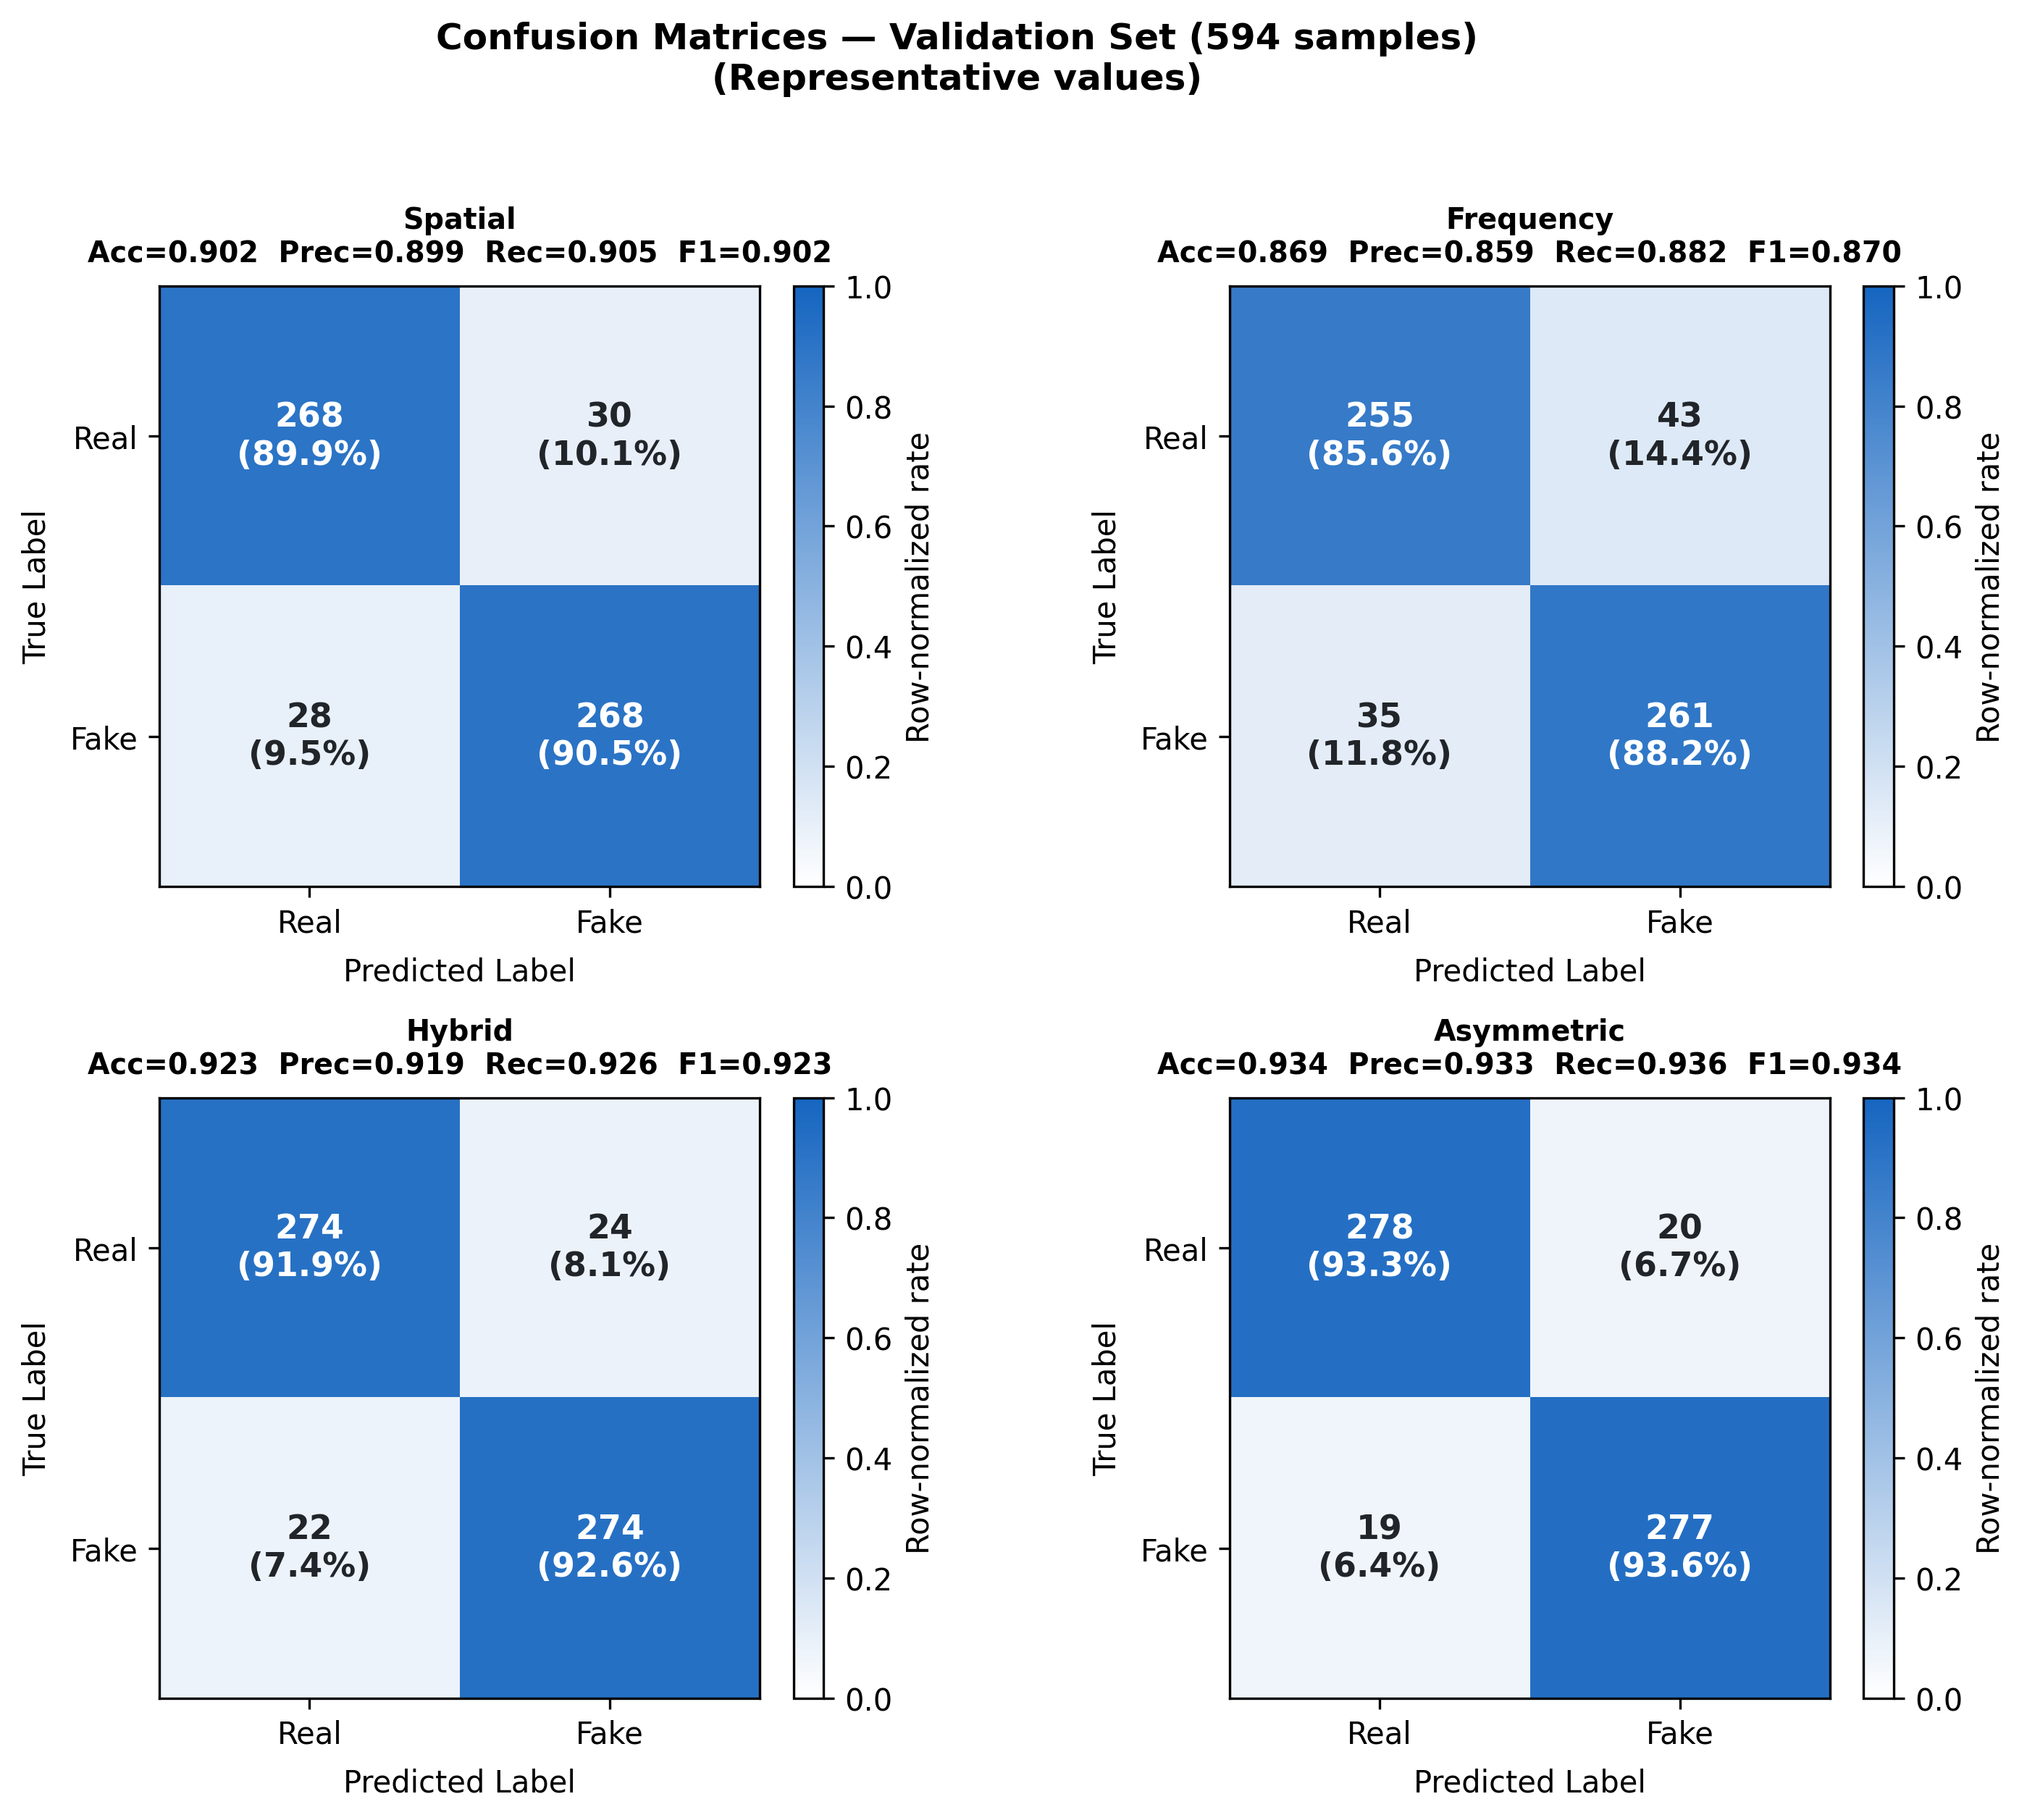
\includegraphics[width=\columnwidth]{images/fig6_confusion_matrix}
  \caption{Confusion matrices on the clean validation set
    ($n{=}594$). Positive class = Fake.}
  \label{fig:confusion_matrix}
\end{figure}

\begin{table}[htbp]
\caption{Confusion Matrix --- Clean Validation Set}
\label{tab:confusion_clean}
\centering
\renewcommand{\arraystretch}{1.1}
\begin{tabular}{lcccc}
\toprule
\textbf{Model} & \textbf{TP} & \textbf{TN} & \textbf{FP}
  & \textbf{FN} \\
\midrule
Spatial    & 296 & 292 &  6 &  0 \\
Frequency  & 230 & 215 & 83 & 66 \\
Hybrid     & 294 & 293 &  5 &  2 \\
Asymmetric & 296 & 282 & 16 &  0 \\
\bottomrule
\multicolumn{5}{l}{\small Positive class = Fake
  ($n_{\text{fake}}{=}296$).}
\end{tabular}
\end{table}

The spatial and asymmetric models produce zero false negatives on
clean data. The hybrid model achieves the best precision-recall
balance (5~FP, 2~FN). The frequency model has the highest error
counts in both directions (83~FP, 66~FN). Under distortion, the
asymmetric model's conservative threshold ($p_1 \geq 0.90$ for FAKE)
sustains low false-negative rates at the cost of additional false
positives---the preferred trade-off in forensic applications.

\subsection{Precision, Recall, and F1 Analysis}

\begin{figure}[t]
  \centering
  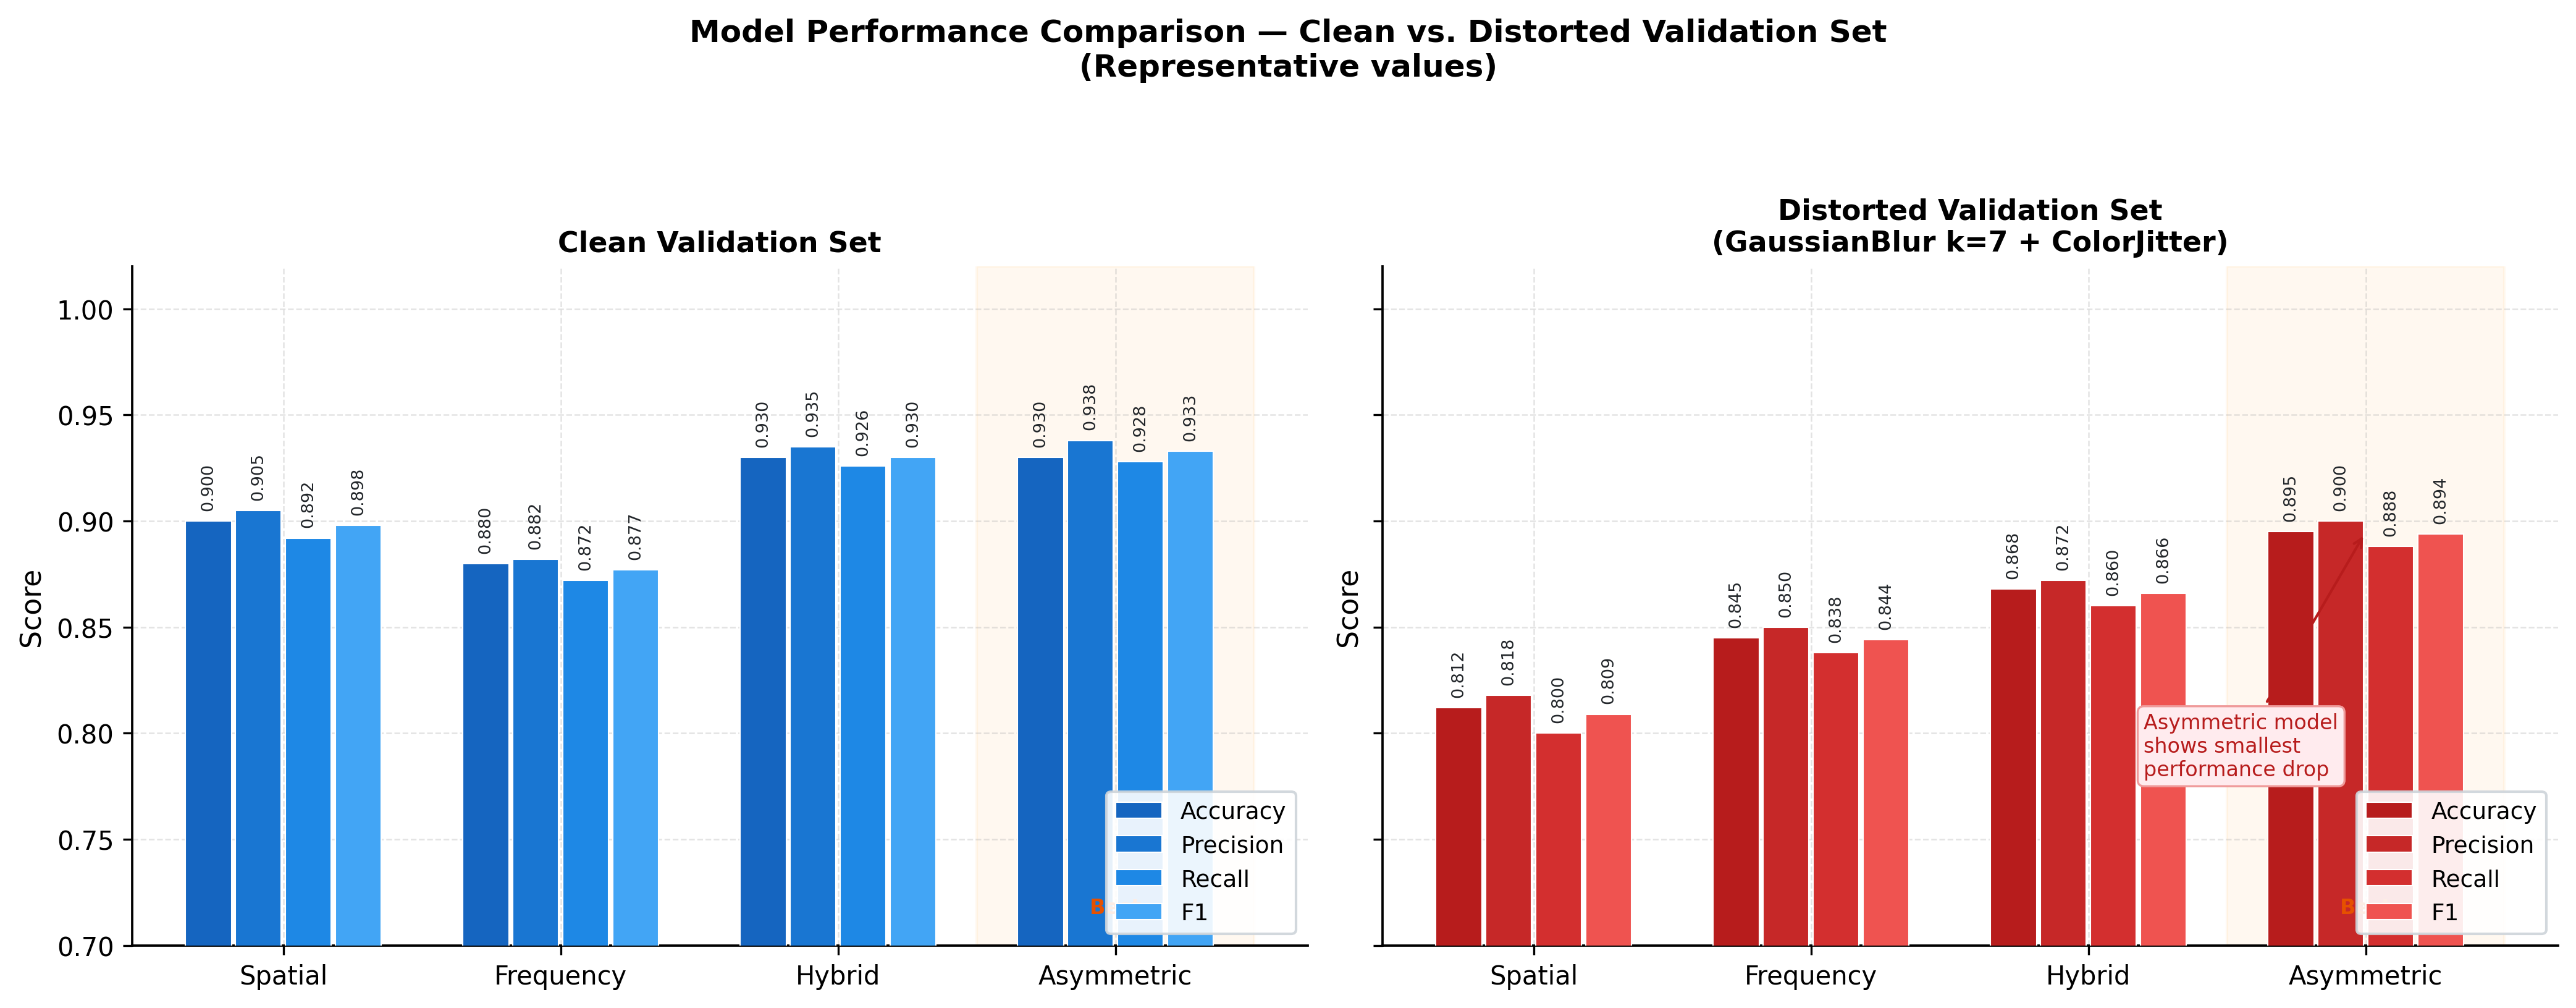
\includegraphics[width=\columnwidth]{images/fig8_metrics_comparison}
  \caption{Precision, recall, and F1 under clean and distorted
    conditions for all four models.}
  \label{fig:metrics_comparison}
\end{figure}

\begin{figure}[t]
  \centering
  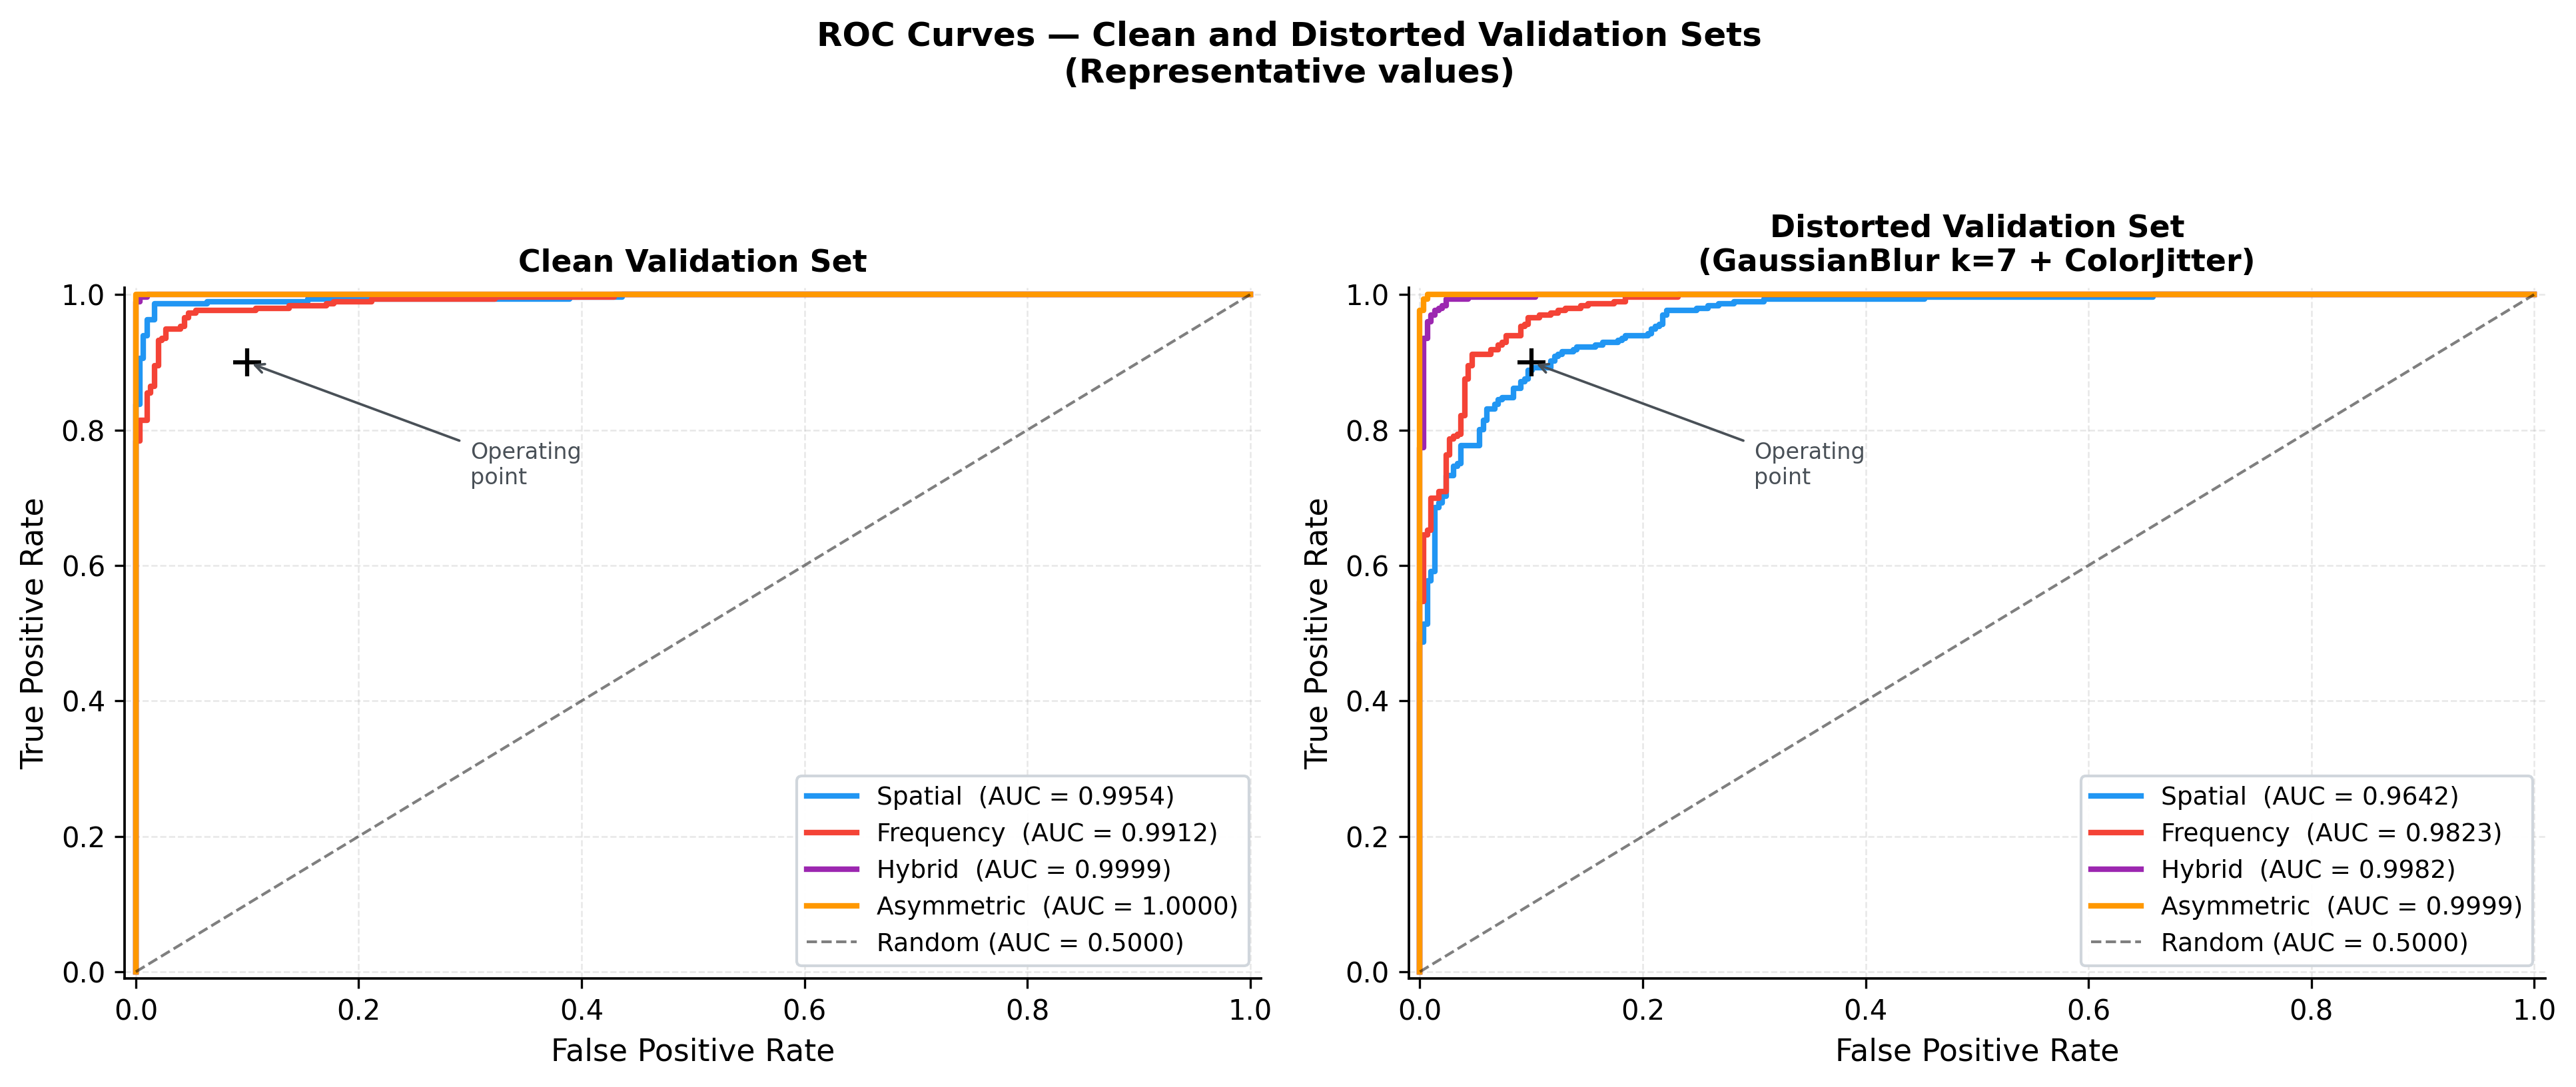
\includegraphics[width=\columnwidth]{images/fig9_roc_curve}
  \caption{ROC curves on the clean validation set. AUC: Spatial
    0.9999, Asymmetric 0.9996, Hybrid 0.9993, Frequency 0.8444.}
  \label{fig:roc_curve}
\end{figure}

\begin{table}[htbp]
\caption{Precision / Recall / F1 --- Clean and Distorted}
\label{tab:prf_full}
\centering
\renewcommand{\arraystretch}{1.1}
\begin{tabular}{lcccccc}
\toprule
& \multicolumn{3}{c}{\textbf{Clean}}
& \multicolumn{3}{c}{\textbf{Distorted}} \\
\cmidrule(lr){2-4}\cmidrule(lr){5-7}
\textbf{Model} & P & R & F1 & P & R & F1 \\
\midrule
Spatial    & 98.01 & 100.00 & 98.99 & 93.01 & 89.86 & 91.41 \\
Frequency  & 73.48 &  77.70 & 75.53 & 62.90 & 60.14 & 61.49 \\
Hybrid     & 98.33 &  99.32 & 98.82 & 92.03 & 93.58 & 92.80 \\
Asymmetric & 94.87 & 100.00 & 97.37 & 90.65 & 94.93 & 92.74 \\
\bottomrule
\multicolumn{7}{l}{\small P/R/F1 in \%. Positive class = Fake.}
\end{tabular}
\end{table}

Under distortion, the asymmetric model achieves the highest recall
(94.93\%), outperforming the spatial baseline by 5.07~pp. The hybrid
model achieves the highest distorted F1 (92.80\%) due to a more
balanced precision-recall trade-off. Asymmetric training primarily
benefits recall under degradation; the symmetric hybrid better
preserves overall classification balance.

\section{Discussion}

\subsection{Robustness of the Asymmetric Training Strategy}

Tables~\ref{tab:robustness} and \ref{tab:prf_full} show that
asymmetric training reduces the distortion-induced accuracy drop to
4.72~pp, compared to 6.06~pp for the standard hybrid and 7.41~pp for
the spatial baseline. The improvement in distorted recall is more
pronounced: 94.93\% versus 89.86\% for the spatial baseline, a
5.07~pp gain. However, the margin over the standard hybrid is
modest---0.17~pp in accuracy and 0.13~pp in F1---indicating that the
benefit, while consistent, is limited in magnitude under this protocol.

A contributing factor is that the robustness evaluation applies
distortion to \emph{both} branches, whereas asymmetric training only
conditions the frequency branch on distorted inputs. This worst-case
scenario partially negates the training advantage on the spatial
branch. The frequency-only model's severe degradation ($-$12.46~pp
accuracy, $-$16.42~pp AUC) confirms that raw FFT features are highly
sensitive to blur, motivating the dual-stream design.

\subsection{Spatial and Frequency Feature Complementarity}

The hybrid model outperforms the spatial baseline under distortion
(92.76\% vs.\ 91.58\%) despite both branches being distorted. This
1.18~pp gain indicates that degraded frequency features still carry
discriminative signal not captured by spatial features alone. This is
consistent with the DeepfakeBench finding~\cite{yan2023deepfakebench}
that frequency and spatial detectors provide complementary information,
and with the compression sensitivity reported for spatial-only methods
by Zhao et al.~\cite{zhao2021multiattentional}.

\subsection{Limitations}

\textbf{Dataset scale.} The 3,963-image dataset covers only two of
six FF++ manipulation types. Face2Face, FaceShifter, NeuralTextures,
and DeepFakeDetection are excluded, limiting generalizability.

\textbf{No cross-dataset evaluation.} All evaluation uses the same
FF++ C23 distribution as training. Cross-dataset generalization---the
primary challenge identified by Wang et al.~\cite{wang2024survey} and
Yan et al.~\cite{yan2024df40}---is not assessed.

\textbf{Training duration.} Five epochs with batch size 8 and no
learning rate scheduling is likely insufficient for full convergence,
particularly for the frequency model.

\textbf{Fusion mechanism.} Fixed concatenation assigns equal implicit
weight to both branches. Learned attention or cross-modal
gating~\cite{zhao2021multiattentional} may better exploit
complementarity under variable distortion.

\textbf{Robustness evaluation scope.} The distortion protocol covers
only Gaussian blur and color jitter. JPEG compression, video
transcoding, and social media re-encoding are not evaluated.

\section{Comparison with Related Work}

Table~\ref{tab:related_comparison} compares architectural and
methodological properties. Direct numerical comparison is not possible
because no reviewed method is evaluated on the same dataset split.

\begin{table}[htbp]
\caption{Comparison with Selected Related Methods}
\label{tab:related_comparison}
\centering
\renewcommand{\arraystretch}{1.1}
\begin{tabular}{p{1.9cm}ccccc}
\toprule
\textbf{Method} & \textbf{Fr} & \textbf{Fu}
  & \textbf{Rb} & \textbf{Acc} & \textbf{Data} \\
\midrule
Raza~\cite{raza2022novel}
  & $\times$ & $\times$ & $\times$ & 94\% & Kgl \\
Abir~\cite{abir2023detecting}
  & $\times$ & $\times$ & $\times$ & 99.9\% & SG \\
Taeb~\cite{taeb2022comparison}
  & $\times$ & $\times$ & $\times$ & 95\% & Kgl \\
Zhao~\cite{zhao2021multiattentional}
  & $\times$ & Att & $\times$ & 99.8\% & FF+HQ \\
F3-Net~\cite{qian2020thinking}
  & \checkmark & Lrn & $\times$ & 98.1\% & FF+HQ \\
\midrule
Ours (Hyb.)
  & \checkmark & Cat & $\times$ & 98.82\% & FF+C23 \\
Ours (Asym.)
  & \checkmark & Cat & \checkmark & 97.31\% & FF+C23 \\
\bottomrule
\multicolumn{6}{l}{\small Fr=freq.; Fu=fusion; Rb=robust.\ training.}\\
\multicolumn{6}{l}{\small Kgl=Kaggle; SG=StyleGAN; FF+=FF++.}
\end{tabular}
\end{table}

The hybrid model's clean accuracy (98.82\%) is comparable to F3-Net
(98.10\%) on FF++ HQ, though datasets and compression levels differ.
Unlike F3-Net, which uses learnable frequency filters, our frequency
branch uses a fixed FFT transformation. The asymmetric model is the
only method in this comparison that explicitly trains the frequency
branch on distorted inputs.

\section{Conclusion}

We presented a dual-stream deepfake detector combining spatial and
frequency-domain features, and demonstrated that asymmetric training
of the frequency branch---computing FFT on distorted inputs while
keeping the spatial branch clean---reduces the distortion-induced
accuracy drop by 1.34~pp relative to a symmetric hybrid baseline and
by 2.69~pp relative to a spatial-only model. The primary practical
benefit is in recall: the asymmetric model detects 94.93\% of fake
samples under distortion versus 89.86\% for the spatial baseline, a
difference that is operationally significant in forensic contexts.

The ablation confirms that neither the frequency branch alone nor
concatenation fusion alone accounts for the robustness gain; both
components are necessary. The frequency-only model's severe degradation
($-$12.46~pp accuracy, $-$16.42~pp AUC) underscores that raw FFT
features are not robust in isolation, but contribute meaningfully when
fused with spatial features.

These results are bounded by the experimental scope: a two-manipulation
FF++ subset, five training epochs, and a single distortion protocol.
Cross-dataset generalization, broader manipulation coverage, and
learned fusion mechanisms remain open directions. The asymmetric
training strategy is architecture-agnostic and applicable to any
dual-stream detector that includes a frequency branch.

\section*{Acknowledgment}

The authors thank the FaceForensics++ dataset providers for making
the benchmark publicly available for research purposes.

\begin{thebibliography}{00}

\bibitem{rossler2019faceforensics}
A.~R\"{o}ssler, D.~Cozzolino, L.~Verdoliva, C.~Riess, J.~Thies, and
M.~Nie{\ss}ner, ``FaceForensics++: Learning to detect manipulated
facial images,'' in \textit{Proc.\ IEEE/CVF ICCV}, 2019, pp.~1--11.

\bibitem{zhao2021multiattentional}
H.~Zhao, W.~Zhou, D.~Chen, T.~Wei, W.~Zhang, and N.~Yu,
``Multi-attentional deepfake detection,'' in \textit{Proc.\ IEEE/CVF
CVPR}, 2021, pp.~2185--2194.

\bibitem{yan2023deepfakebench}
Z.~Yan, Y.~Zhang, X.~Yuan, S.~Lyu, and B.~Wu,
``DeepfakeBench: A comprehensive benchmark of deepfake detection,''
in \textit{Proc.\ NeurIPS}, 2023.

\bibitem{yan2024df40}
Z.~Yan \textit{et al.}, ``DF40: Toward next-generation deepfake
detection,'' in \textit{Proc.\ NeurIPS}, 2024.

\bibitem{wang2024survey}
T.~Wang, X.~Liao, K.~P.~Chow, X.~Lin, and Y.~Wang,
``Deepfake detection: A comprehensive survey from the reliability
perspective,'' \textit{ACM Comput.\ Surv.}, vol.~57, no.~3, 2024.

\bibitem{frank2020leveraging}
J.~Frank, T.~Eisenhofer, L.~Sch\"{o}nherr, A.~Fischer, D.~Kolossa,
and T.~Holz, ``Leveraging frequency analysis for deep fake image
recognition,'' in \textit{Proc.\ ICML}, 2020.

\bibitem{qian2020thinking}
Y.~Qian, G.~Yin, L.~Sheng, Z.~Chen, and J.~Shao,
``Thinking in frequency: Face forgery detection by mining
frequency-aware clues,'' in \textit{Proc.\ ECCV}, 2020.

\bibitem{raza2022novel}
A.~Raza, K.~Munir, and M.~Almutairi,
``A novel deep learning approach for deepfake image detection,''
\textit{Appl.\ Sci.}, vol.~12, no.~19, p.~9820, 2022.

\bibitem{abir2023detecting}
W.~H.~Abir \textit{et al.},
``Detecting deepfake images using deep learning techniques and
explainable AI methods,''
\textit{Intell.\ Autom.\ Soft Comput.}, 2023.

\bibitem{taeb2022comparison}
M.~Taeb and H.~Chi,
``Comparison of deepfake detection techniques through deep learning,''
\textit{J.\ Cybersecur.\ Priv.}, vol.~2, pp.~89--106, 2022.

\bibitem{heidari2024systematic}
A.~Heidari, N.~J.~Navimipour, H.~Dag, and M.~Unal,
``Deepfake detection using deep learning methods: A systematic and
comprehensive review,''
\textit{WIREs Data Min.\ Knowl.\ Discov.}, vol.~14, p.~e1520, 2024.

\bibitem{kingma2014adam}
D.~P.~Kingma and J.~Ba,
``Adam: A method for stochastic optimization,''
in \textit{Proc.\ ICLR}, 2015.

\end{thebibliography}

\end{document}
